\documentclass[lettersize,journal]{IEEEtran}
% \documentclass[draftclsnofoot,onecolumn]{IEEEtran}
% \documentclass[draft]{article}  %draft
\usepackage{amsmath,amsfonts}
\usepackage{algorithmic}
\usepackage{algorithm}
\usepackage{array}
\usepackage[caption=false,font=normalsize,labelfont=sf,textfont=sf]{subfig}
\usepackage{textcomp}
\usepackage{stfloats}
% \usepackage{url}
\usepackage{verbatim}
\usepackage{graphicx}
\usepackage{cite}  % [doi=false, url=false] BUG？
\usepackage[backref]{hyperref}
\usepackage{multirow}%\multicolumn{}{}{}

% \usepackage[style=ieee,doi=false,isbn=false,url=false,eprint=false]{BibTeX}

\hyphenation{op-tical net-works semi-conduc-tor IEEE-Xplore}
% updated with editorial comments 8/9/2021

\begin{document}

\title{
Explainable operator attention network: an explainable neural network for bearing fault diagnosis via dynamic sparse operator attention
} 

%%%%%%%%%%%%%%%%%%%%%%%% 

\author{Qi Li, \textit{Graduate Student Member, IEEE}, Wenyang Hu, Qijian Lin, Hua Li, \textit{Senior Member, IEEE}, 

Zhaoye Qin, \textit{Member}, IEEE, Fulei Chu

\thanks{This research was supported by the Science Center for Gas Turbine Project (Grant No. P2022-B-III-002–001).(Corresponding author: Zhaoye Qin.)

Qi Li, Wenyang Hu, Qijian Lin, Zhaoye Qin, Fulei Chu are with State Key Laboratory of Tribology, Department of Mechanical Engineering, Tsinghua University, Beijing, China (email:liq22@tsinghua.org.cn;
hwy20@mails.tsinghua.edu.cn;
linqj22@mails.tsinghua.edu.cn;
qinzy@mail.tsinghua.edu.cn;
chufl@mail.tsinghua.edu.cn).

Hua Li is with State Key Laboratory of Tribology, Department of Mechanical Engineering, Tsinghua University, Beijing, China and State Key Laboratory of Public Big Data, Guizhou University, Guiyang 550025, China (email: lihua.41@163.com)}
}
%%%%%%%%%%%%%%%%%%%%%%%%%%%%
        % <-this % stops a space


% The paper headers
% \markboth{Journal of \LaTeX\ Class Files,~Vol.~14, No.~8, August~2021}%
% {Shell \MakeLowercase{\textit{et al.}}: A Sample Article Using IEEEtran.cls for IEEE Journals}

% \IEEEpubid{0000--0000/00\$00.00~\copyright~2021 IEEE}
% Remember, if you use this you must call \IEEEpubidadjcol in the second
% column for its text to clear the IEEEpubid mark.

\maketitle

\begin{abstract}

 Explainable AI has gained significant traction across various industrial sectors, particularly in intelligent fault diagnosis. However, dynamically integrating domain expertise with neural networks to enhance explainability poses a challenge. Therefore, this study presents a novel eXplainable Operator Attention Network (XOAN), which capitalizes on an explainable Expert Knowledge Dictionary (EKD) with signal processing and statistical features for analyzing signals. Then, a novel Dynamic Sparse Operator Attention (DSOA) module is proposed to dynamically identify critical expert knowledge through a top-k attention mechanism. By incorporating DSOA into an operator attention block, XOAN enables seamless end-to-end learning and inference, optimizing diagnostic capabilities. Case studies showcase the effectiveness and explainability of XOAN, illustrating how it allows neural networks to select the most relevant expert operators. Ultimately, XOAN significantly advances the reliability of knowledge-informed intelligent diagnostic learning systems, making it a valuable contribution to the field of explainable AI and fault diagnosis.



%%

% The advent of Industry 4.0 has heightened the demand for the interpretability of intelligent diagnostics, especially for high-risk industrial assets. However, the comprehensive interpretation of neural networks remains inadequately explored. To address this challenge and develop a fully explainable network, we propose a transparent operator network incorporating a parameterized signal operator node. 
% The advent of Industry 4.0 has heightened the demand for the interpretability of intelligent diagnostics, especially for high-risk industrial assets. However, the comprehensive interpretation of neural networks remains inadequately explored. To address this challenge and develop a fully explainable network, we propose a transparent operator network incorporating a parameterized signal operator node. 
% This node is realized by a learnable Morlet wavelet operator in frequency domain with signal-wise gated matrix and skip connection. By stacking multi-channel and multi-layered nodes as signal operator layers, along with incorporating statistical features and a linear classifier, all modules are physically understandable. A case study demonstrates that despite having fewer parameters, the proposed model achieves better diagnosis performance. Furthermore, the learnable filters, fault signature enhancement, and physically understandable features demonstrate the transparency of the proposed model, indicating that it offers  a promising tool for constructing a knowledge-informed and fully explainable industrial decisions. 

\end{abstract}

\begin{IEEEkeywords}
Intelligent fault diagnosis, operator attention, expert knowledge, signal processing, XAI, rotating machinery.
\end{IEEEkeywords}

%%

\section{Introduction}

% \subsection{background}
\IEEEPARstart{M}{odern} AI systems are commonly perceived as black boxes due to their lack of transparency in behavior and decision-making processes  \cite{Rong2024}. Explainable AI (XAI) is deemed essential for the continuous advancement of AI research across various fields including medicine \cite{Holzinger2022}, industry \cite{Li2023} and automobiles \cite{Dong2023}. The explainablity of a model is essential for the effective implementation of AI, particularly in critical domains such as industrial asset fault diagnosis \cite{Li2024}. Fault diagnosis is a valuable tool for ensuring the safe operation of industrial systems and minimizing avoidable maintenance costs due to routine shutdowns \cite{henriquezReviewAutomaticFault2014, wang_coarse--fine_2023}. Given its growing importance in modern society, if AI-assisted diagnostic methods lack explainability, industries may not trust the decision-making processes, leading to a crisis of trustworthiness. In the present context, there exist three primary approaches of fault diagnosis: expert knowledge-based fault diagnosis, methods employing deep learning techniques, and explainable approaches that combine knowledge with deep learning methods. 

 

% \subsection{Bearing Fault Diagnosis}
\subsubsection{Fault diagnosis based on expert knowledge}
Fault diagnosis serves an important role in pursuing the relationship between monitoring data and the health states of machines, which is a widely concerned issue in machine health management \cite{lu_edge_2023}. Diagnostic experts utilize their knowledge and tools to interpret these signals, leading to the diagnosis results that inform the health state of the machinery \cite{Lei2020}. Traditional fault diagnosis methods involve signal processing and feature extraction of monitoring data collected by sensors as shown in Fig. \ref{idea} (a).  These methods commonly involve wavelet transform \cite{Yan2023}, mode decomposition methods and feature extraction \cite{miao_feature_2023}. For instance,  Miao et al. \cite{miao_feature_2023} proposed a feature mode decomposition theory as feature extraction to decompose the different modes by the designed adaptive finite-impulse response filters guided by the correlated Kurtosis, where Kurtosis feature is suitable to detect transient abnormal signals in the presence of strong additive noise \cite{antoni_spectral_2006}. 

\begin{figure}[htbp] 
\centerline{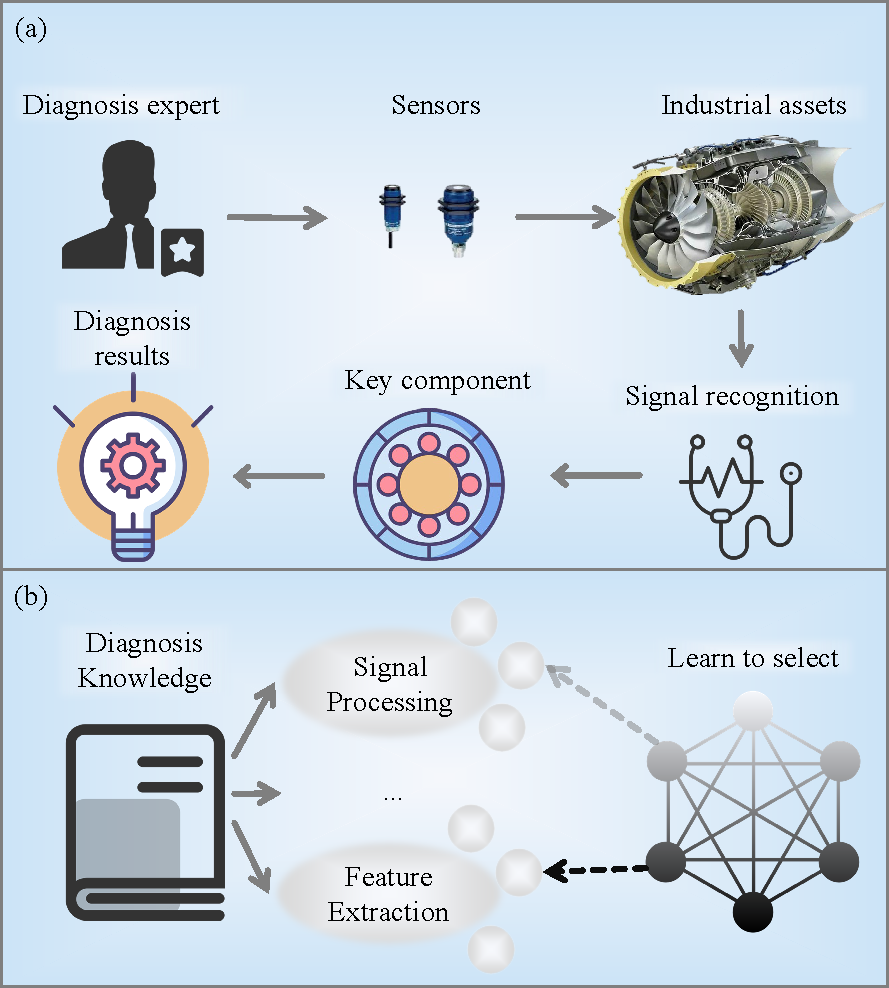
\includegraphics[width=0.95\linewidth]{figs/idea3.pdf}}
\caption{The motivation of XOAN. (a) Traditional fault diagnosis with expert knowledge, (b) XOAN aims to incorporate expert knowledge into neural networks by employing operator attention to facilitate the learning process of selecting expert knowledge. }
\label{idea}
\end{figure}

\subsubsection{Deep learning-based method}
In the era of AI, many tasks involve deep learning to directly learn the relationship from monitored signals to the health state of the machine. For example, Gao et al \cite{Gao2021} proposed a novel weak fault feature extraction and diagnosis method using multi-channel continuous wavelet transform and a convolution-feature-based recurrent neural network. Li et al. \cite{Li2023} utilized GAN to achieve cross-domain generalization.

\subsubsection{Knowledge-informed explainable intelligent fault diagnosis}
Recently, many knowledge-informed diagnostic methods have emerged, balancing both performance and explainability \cite{deng_physics-informed_2023}. Wang et al. \cite{wangPhysicallyInterpretableWaveletguided2024} proposed a physically interpretable wavelet-guided network (WaveGNet) with deep frequency separation, providing a basis and physical meaning for the discrete wavelet transform (DWT). Li et al. \cite{liWaveletKernelNetInterpretableDeep2020a} designed a continuous wavelet convolutional (CWConv) layer to replace the first convolutional layer of the standard CNN. Qin et al. \cite{qin_vwm-dcrnn_2023} proposed a diagnostic method using variational mode decomposition and a dual model of convolutional recurrent neural network to identify faults in insulated gate bipolar transistors. Ha et al. \cite{ha_domain_2023} utilized a health data map to visually display the vibration signal of a planetary gearbox as an image-like matrix, aiding in the observation of fault-related characteristics. Su et al. \cite{su_knowledge-informed_2024} introduced a knowledge-informed deep network that leverages knowledge-based features along with a data-driven constrained Gaussian process for precise bearing fault prediction. Ni et al. \cite{ni_physics-informed_2023} developed a physics-informed residual network designed to learn the inherent physics in both training and testing data. This network includes a physical modal-property-dominant-generated layer and a domain-conversion layer, providing a physically consistent solution for imperfect data.

% \subsection{Proposed method}
While the work mentioned above has achieved notable success, it is important to acknowledge that the current methods also have some limitations.
\begin{itemize}
    \item Firstly, some black box modules remain unexplainable, such as the randomly parameterized convolutional layers that users may find challenging to understand \cite{Li2024_TON}.
    \item Moreover, the knowledge-informed network necessitates the manual selection of expert knowledge modules for each case. This approach relies on pre-configured fixed modules, making it difficult to determine the appropriate knowledge to incorporate into the model design.
\end{itemize}

To address these issues, we propose an eXplainable Operator Attention Network (XOAN), considering the possibility of utilizing neural networks to learn how to focus on various expert knowledge. This approach can provide explainable feedback to the researcher, as illustrated in Fig. \ref{idea} (b). In the XOAN framework, an expert knowledge dictionary (EKD) is initially constructed for signals, incorporating signal processing and feature extraction techniques, which can be utilized in subsequent model learning. Furthermore, a Dynamic Sparse Operator Attention (DSOA) module was developed to dynamically learn and select the most critical expert knowledge using top-k attention mechanisms which contributes to achieving explainable models. Finally, by leveraging the DSOA, an Operator Attention block was designed and integrated into the model to facilitate end-to-end learning and inference for diagnostics. 
The contributions of this paper can be summarized as follows: 
\begin{itemize}
    \item   To achieve explainable fault diagnosis,  a XOAN model is introduced, incorporating expert knowledge through neural networks to determine the most appropriate expert knowledge dictionary (EKD) for human comprehension.
    \item   Within XOAN, a explainable operator (XOA) block is presented along with the Dynamic Sparse Operator Attention (DSOA) and feature pooling (FP) to dynamically identify and choose expert operators according to particular signals.
    \item Case studies involve the application of signal processing and feature extraction operators in the realm of intelligent fault diagnosis, showcasing its potential by adaptively employing attention to select interpretable operators, thus laying a stronger foundation for trustworthy industrial applications. 

% \begin{itemize}
    % \item Signal dataset
    % \item Signal dataset generalization capability
    % \item Multiple signal dataset result
% \end{itemize}
 
\end{itemize}

The rest of this paper is structured as follows: Section II provides a preliminary to expert knowledge in bearing fault diagnosis and attention. Section III introduces the explainable operator attention network with dynamic sparse operator attention. Section IV outlines the experimental setup, results, and discussion. Section V concludes with final remarks and future research directions.

\section{Preliminary}

\subsection{Expert knowledge in Bearing fault diagnosis}


\subsubsection{Filtering}
Bearing fault diagnosis has evolved over decades, with the classic approach involving filtering the original bearing signal followed by envelope analysis \cite{Randall2011}, and other related pattern recognition methods \cite{WORDEN20114}. One exemplary filtering method is the FIR filter, which aims to eliminate noise and enhance specific features of the signal. For a real signal $x(n)$, the response of the FIR system can be formulated via convolution operator as \cite{Rui2024},
\begin{equation}
    y(n)=h(n)*x(n)=\sum_{m=0}^{L-1}h(m)x(n-m),
\end{equation}
where $h(n)$ represents the filter coefficient, incorporating frequency waves such as Hanning, Blackman windows. To locate the typical fault signature, the wavelet filter operator (WFO) \cite{Li2024_TON} is designed to dynamically learn the center frequency and bandwidth to capture the feature of the monitoring signal, which can be formulated as:
\begin{equation}\label{eq.FO}
    \left(\mathcal{K}(\theta) \mathbf{x}\right)=\mathcal{F}^{-1}\left(R_\theta(w) \cdot\left(\mathcal{F} \mathbf{x}\right)\right), \quad 
\end{equation}
where $\mathcal{F}$ denotes the Fourier transform, $\mathcal{F}^{-1}$ denotes the inverse Fourier transform. The wavelet is chosen as Morlet and its frequency domain can be denoted as:
\begin{equation}
    R_\theta(w)=e^{-(\omega-2\pi f_c)^{2}/(4 f_b ^{2})} \label{eqfilter},
\end{equation}
where $\theta = \{f_b,f_c\}$ represent the parameterized center frequency and bandwidth, respectively.

\subsubsection{Envelope analysis}
To extract clearer diagnostic information, the prepossessed signals were demodulated to obtain the envelope signal by envelope analysis, which performs to detect characteristic fault frequencies such as Ball Pass Frequency Outer (BPFO), Ball Pass Frequency Inner (BPFI), Fundamental Train Frequency (FTF), and Ball Spin Frequency (BSF) \cite{Randall2011}. 

By constructing an imaginary part orthogonal to the original signal through Hilbert transform, one can extract the analytic signal's magnitude, thereby determining the amplitude variation over time. The Hilbert transform of a signal $x(t)$ is defined as Eq. \ref{eq.HT}:
\begin{equation}\label{eq.HT}
HT(t) = \frac{P}{\pi }\int_{ - \infty }^{ + \infty } {\frac{{x(\tau )}}{{t - \tau }}} {\rm{d}}\tau,
\end{equation}
where $P$ denotes the Cauchy principal value of the integral. Applying the Hilbert transform to the signal $x(t)$ results in its analytic signal $z(t)$, which consists of a real part $x(t)$ and an imaginary part $y(t)$:
\begin{equation}\label{eq2}
z(t) = x(t) + jy(t).
\end{equation}
The magnitude of the analytic signal $|z(t)|$ is the envelope of the signal $x(t)$, which contains information about its amplitude modulation. 

\subsubsection{Feature extraction}
Enhanced signals enable the extraction of their statistical characteristics for signal pattern recognition. These features comprise various sets, as shown in Table \ref{tab:feature sets}, including typical statistical features like mean, variance, peak value, root mean square, kurtosis, crest factor, skewness, etc\cite{badihiComprehensiveReviewSignalBased2022a, leiApplicationsMachineLearning2020d}. These features are commonly used as physical health indicators for machine health monitoring. Additionally, Entropy, a well-known measure in information theory, is extensively employed in machine fault diagnosis. 

Establishing a pipeline of operators for a new machine can be a complex task, as it involves choosing specific features using expert knowledge. This complexity presents a challenge in integrating of this explainable expert knowledge into an adaptable Intelligent Fault Diagnosis (IFD) model. 

\begin{table*}
    \centering
\caption{Features and their semantics}

\captionsetup{justification=raggedright}
\tabcolsep=0.7cm
\label{tab:feature sets}
    \begin{tabular}{lcclll} \hline  
          NO.&Feature name& Equations &  NO.&Feature name&Equations \\ \hline  
          0&Mean& $\frac{1}{N}\sum_{i=1}^{N} x_i$ &  7&Kurtosis&$\frac{\frac{1}{N}\sum_{i=1}^{N} (x_i - \mu)^4}{\sigma^4}$ \\ 
          1
&Std& $\sqrt{\frac{1}{N}\sum_{i=1}^{N} (x_i - \mu)^2}$ &  8&RMS&$\sqrt{\frac{1}{N}\sum_{i=1}^{N} x_i^2}$ \\  
          2
&Var& $\frac{1}{N}\sum_{i=1}^{N} (x_i - \mu)^2$ &  9&Crest Factor&$\frac{\max (x)}{RMS(x)}$ 
\\
          3
&Entropy& $-\sum_{i=1}^{N} p(x_i) \log p(x_i)$ &  10&Skewness&$\frac{\frac{1}{N}\sum_{i=1}^{N} (x_i - \mu)^3}{\sigma^3}$ \\ 
          4
&Max& $\max(x)$ &  11&Clearance Factor&$ \frac{\max (x)}{\frac{1}{N}\sum_{i=1}^{N}|x_i|}$ \\ 
          5
&Min& $\min(x)$ &  12&ShapeFactor&$ \frac{RMS(x)}{\frac{1}{N}\sum_{i=1}^{N}|x_i|}$ 
\\
         6&AbsMean&$\frac{1}{N}\sum_{i=1}^{N} |x_i|$ &  13&Crest Factor Delta&$ \frac{\sqrt{\frac{1}{N}\sum_{i=1}^{N} (x_{i+1} - x_i)^2}}{\frac{1}{N}\sum_{i=1}^{N}|x_i|}$ \\ \hline
    \end{tabular}
\end{table*}

% crest factor delta didn't use

\subsection{Attention }

Attention mechanisms are techniques used to focus on the most important parts of the input data while ignoring less relevant information, which is proposed in 2017 \cite{guo_attention_2022}. These mechanisms mimic the human visual system, which naturally finds salient regions in complex scenes.  A general attention mechanism can be formulated as: 
\begin{equation}
    \text{Attention} = f(g(x), x) ,
\end{equation}
where  $g(x)$ is the attention which corresponds to the process of attending to discriminating regions. $ f(g(x), x)$  processes the input \( x \) based on the attention \( g(x) \). Typically, for self-attention, the process can be described as: first compute the query, key, and value matrices from the input:
\begin{equation}
Q, K, V = \text{Linear}(x).
\end{equation}
Then compute attention scores (ASs) with Softmax and scale factor $\sqrt{d_k}$:
   \begin{equation}
    g(x) = \mathrm{Softmax}(\frac{QK^T}{\sqrt{d_k}}).
   \end{equation}
Finally, compute the output by combining the ASs with the values:
\begin{equation}\label{attention}
f(g(x), x) = g(x)V.
\end{equation}
% In addition to self-attention, there are other types of attention mechanisms including channel attention, spatial attention, temporal attention, branch attention, and hybrid attention among others.

However, there is an urgent need for research on how to enhance the explainability of models, despite the current focus on improving model performance through attention mechanisms. This paper explores the characteristics of attention, which adaptively focus on salient operators, to achieve dynamically explainable models using explainable diagnostic knowledge and tailored attention methods. 


\section{Explainable operator attention network with Dynamic Sparse Operator Attention}

\subsection{The whole model}

We developed an XOAN based on expert knowledge and attention mechanisms to dynamically learn and focus on specific knowledge, thereby enhancing the explainability of model. Specifically, Fig. \ref{fig XOAN} shows the key architecture of the XOAN. The input signal is composed of signals that sensors monitor. The model includes several XOA blocks for signal processing and feature extraction. Within each XOA block, a customized DSOA is employed to dynamically learn and select the expert operator from EKD, providing researchers with feedback on the focus of expert knowledge through the Top-k sparse ASs.

\begin{figure}[htbp]
\centerline{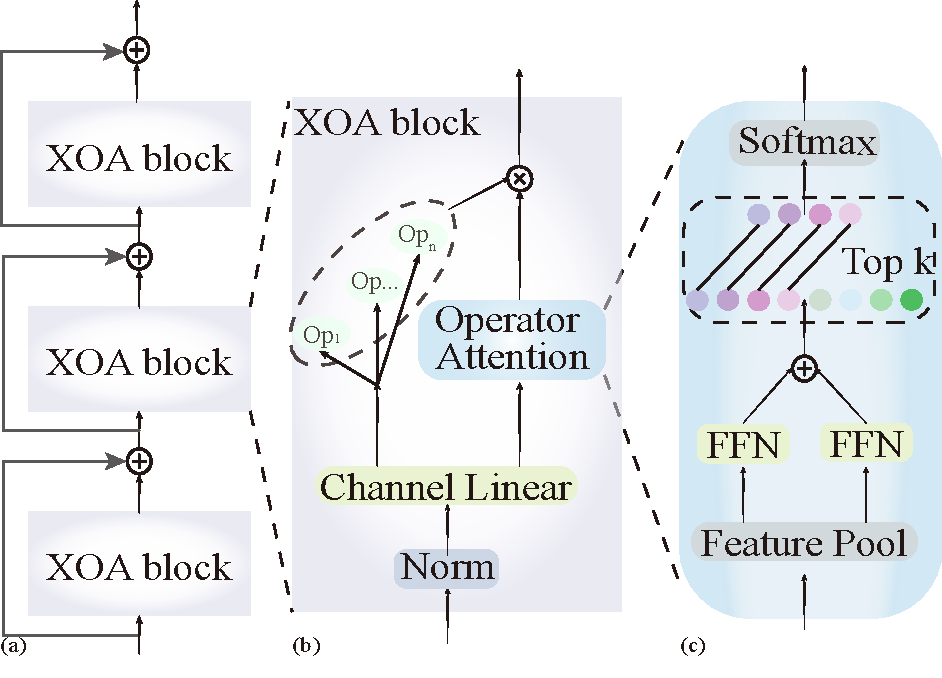
\includegraphics[width=0.9\linewidth]{figs/Model.pdf}}
\caption{The key architecture of XOAN. (a) The proposed XOAN is stacked by XOA block in a residual way, (b) XOA block use Normalization, channel linear layer and dynamic sparse operator attention to learn and select expert operator from EKD, (c) The proposed DSOA use feature pool layer and FFN to learn the top k AS.}
\label{fig XOAN}
\end{figure}

\subsection{Dynamic Sparse Operator Attention}
The input of DSOA is a tensor  $X \in \mathbb{R}^{B \times C \times L}$ with dimensions of batch size, sequence length, and number of channels denoted as $ B, L, C$, respectively. We propose a type of feature pooling (FP) as an extension of the average pooling layer, which can capture multidimensional statistical features of the signal when computing ASs. Specifically, we utilize average pooling $\text{Avgpool}$ and variance pooling $\text{Varpool}$:
\begin{equation}
    \text{Avgpool}(X_{b,c}) = \frac{1}{L} \sum_{i=1}^{L} X_{b,i,c},
\end{equation}
\begin{equation}
    \text{Varpool}(X_{b,c}) =  \frac{1}{L} \sum_{i=1}^{L} \left( X_{b,i,c} - \frac{1}{L} \sum_{j=1}^{L} X_{b,j,c} \right)^2.
\end{equation}

The adaptive average pooling and variance pooling layers compress the signal of each channel into a feature, which is then used to learn inter-channel dependencies through a feed-forward fully connected layer network (FFN) as  
\begin{equation}
    \mathrm{FFN}(X)=\max(0,XW_1+b_1)W_2+b_2.
\end{equation}
By merging the feature information, we obtain the preliminary ASs as:
\begin{equation}
    \text{AS}(X) =\mathrm{FFN}(\text{Avgpool}(X)) + \mathrm{FFN}(\text{Varpool}(X)) .
\end{equation}
To enhance the explainability of model and identify a few crucial attentions for better feedback to researchers, the module should be sparsified. Here, we use the Top-k AS defined as follows: 
\begin{equation}\label{eq.as}
    \text{AS}_{Top-k}(X_i, k) = \left\{ \begin{array}{ll}
\text{Softmax}(X_{i,j}) & \text{if } X_{i,j} \text{ is in Top-k}   \\ % \text{ values in row } i
0 & \text{otherwise} .
\end{array} \right.
\end{equation}
The AS play a crucial role in dynamically selecting the most relevant operators from the EKD, ensuring the model focuses on the most important features by computing and selecting the top-k AS, thereby enhancing both explainability and performance.

\subsection{Expert knowledge dictionary}

Assuming the input signal is $\mathbf{X} \in \mathbb{R}^{B \times C \times L}$, where $B$ represents the batch size, $C$ denotes the number of signal channels, and $L$ is the signal length for each channel. Each signal processing method can be viewed as an operator $OP_i$ that transforms the signal space into an enhanced signal space:

\begin{equation}
    OP_i: \mathbb{R}^{B \times C_1 \times L_1} \to \mathbb{R}^{B \times C_2 \times L_2}, \quad OP \in SP.
\end{equation}
The operators used in this study satisfy $C_1 = C_2$ and $L_1 = L_2$ for network construction convenience. Every feature extraction method can be seen as an operator $OP_i$ that maps the input signal to a feature space:

\begin{equation}
    OP_i: \mathbb{R}^{B \times C \times L} \to \mathbb{R}^{B \times C \times 1}, \quad OP \in FE.
\end{equation}
With the aforementioned sequence of operators, we can construct $EKD_{SP}$ and $EKD_{FE}$:

\begin{equation}
\begin{split}
    EKD_{SP,FE} = 
    {\{\mathcal{P}(OP_i): OP_i}\}_i^{N}, \quad OP_i \in \{SP, FE\},
\end{split}
\end{equation}
where $\mathcal{P}(OP_i)$ represents the semantic attributes or characteristics of operator $OP_i$. With these operators and their semantic attributes, an expert knowledge dictionary is constructed for signal processing and feature extraction operations, facilitating expert comprehension at a later stage.

The selection of signal processing and feature extraction module for constructing the EKD in this paper is based on their proven effectiveness and interpretability in the field of fault diagnosis \cite{liDeepExpertNetwork2024, leiApplicationsMachineLearning2020d}. The criteria for selecting these methods include:

\begin{itemize}
    \item \textbf{Relevance to Fault Diagnosis}: The methods chosen should have direct applications in diagnosing faults in rotating machinery. This paper uses Eq. \ref{eq.FO} and Eq. \ref{eq.HT} for signal processing and statistical features in Table \ref{tab:feature sets} for feature extraction, which are commonly used in bearing fault diagnosis.
    \item \textbf{Proven Effectiveness}: The module should have demonstrated success in previous research and practical applications. The goal of DSOA is to dynamically select the most relevant operators from the EKD, ensuring the model focuses on the most important features.
    \item \textbf{Explainability}: The selected methods should provide clear and understandable results that can be easily interpreted by experts. This is crucial for the explainability aspect of the model.
\end{itemize}

% While the methods included in the EKD represent a comprehensive set of existing expert knowledge, it is acknowledged that the field is continuously evolving, and new methods are being developed. Therefore, the EKD can also be updated to incorporate new advancements. let \( EKD_t \) be the EKD at time \( t \). As new methods \( OP_{new} \) are developed, they can be incorporated into the EKD as follows:
% \begin{equation}
%     EKD_{t+1} = EKD_t \cup \{ OP_{new} \},
% \end{equation}
% where \( \cup \) denotes the union of the existing EKD and the new methods. This ensures that the EKD remains up-to-date with the latest advancements in the field. The dynamic nature of the proposed model allows it to adapt and focus on the most relevant features, mitigating some of the risks associated with an evolving EKD. The significance of establishing the EKD lies in its ability to integrate domain expertise into the model, enhancing its interpretability and reliability. By leveraging expert knowledge, the model can provide more meaningful and trustworthy diagnostic results, which is crucial for industrial applications where decision-making based on AI models needs to be transparent and justifiable.




\subsection{XOA block }
To utilize the DSAO effectively, the initial step involves standardizing the signal scales of different channels. This process of standardization is a common practice in deep learning, aiming to normalize each channel independently:
\begin{equation}
\tilde X = SN({X_c}) = \frac{{{X_c} - {\mu _c}}}{{\sqrt {\sigma _c^2 + \epsilon} }},
\end{equation}
where ${\mu _c} = \frac{1}{L}\sum\nolimits_{l = 1}^L {{X_{c,l}}} $ represents the mean of $X$ in $C$ channel, ${\sigma _c} = \frac{1}{L}\sum\nolimits_{l = 1}^L {({X_{c,l}- {\mu _c}})}$ denotes the standard deviation of $X$ in each channel and $L$ denotes the number of sample points of each channel.  Similar to the FFN within the attention mechanism, the signals from different channels go through a channel linear layer to interact with signals from other channels and produce the $V$ of Eq. \ref{attention}. These attention values are calculated as the channel-wise product of the output of the Linear layer and a specific operator function from $EKD$, denoted as $OP$, applied to the input signal.  
\begin{equation}
    V = OP \circ Linear(X)
\end{equation}
where $V \in \mathbb{R}^{B \times C \times L} $ and  $\text{AS}_{Top-k}(X_i, k) \in \mathbb{R}^{B \times C \times 1 }$  in Eq. \ref{eq.as}. Therefore, the output of XOA block is
\begin{equation}
    Y = \text{AS}_{Top-k}(X_i, k) \times  V
\end{equation}
where $\times$ represents element-wise multiplication across channels. This AS can be understood as the focus on particular expert operators. Higher ASs indicate a preference for selecting those operators, which holds significant implications for researchers in industrial applications. In this paper, we utilize four $XOA_{SP}$ blocks with  $EKD_{SP}$ and one $XOA_{FE}$ block with $EKD_{FE}$.

\subsection{Optimization} 
In general, for IFD, there are operators for signal processing and operators for feature extraction. In this context, the $EKD_{SP}$ module employs Eq. \ref{eq.FO} and Eq. \ref{eq.HT}, , while the $EKD_{FE}$ utilizes classical features in the feature sets in Table \ref{tab:feature sets}. After extracting features $F$, a multiclass classification is performed using a Softmax classifier:
\begin{align}
    Y = \text{Softmax}(W_{\sigma}{F})\label{classifier layer}.
\end{align}
The loss function employed in this study is the classical cross-entropy (CE), defined as follows: 
\begin{align}
    \mathcal{L}(P(y),{P_{W,\theta }}(\tilde y|x)) =  - \frac{1}{N} {\sum\limits_{i = 1}^N {P({y_i})\log {P_{W,\theta }}({{\tilde y}_i}|{x_i})} } 
\end{align}
where $W$ is the weight in the FFN and channel linear layer, $\theta$ is the parameters in the WFO respectively.  Then we apply the l1 norm of $W$ to induce sparsity across the entire connection as
\begin{align}
   \zeta (W) = ||W||_1.
\end{align}
Therefore, the final optimization goal optimized by stochastic gradient decent  \cite{Kingma2015} is:
\begin{align}
\label{target}
    \left( {{W^*},{\theta ^*}} \right) = \mathop {\arg \min }\limits_{(W ,\theta )} (\mathcal{L}(W ,\theta ) + \gamma \zeta (W))
\end{align}
 where the $\gamma$  is the trade-off between CE and L1 regularization. 

\section{Case studies}
% \section{Case study}
\subsection{Dataset setting}\label{section.setting}
\subsubsection{Dataset 1: vibration and Piezoelectric signal}
% \subsubsection{vibration and Piezoelectric signal}

We employ a self-powered condition monitoring dataset obtained using a piezoelectric energy harvester in our lab as shown in Fig. \ref{fig3} \cite{zhang_piezoelectric_2022}. The dataset contains voltage signals from four health conditions: normal (Nor), inner race fault (IF), ball fault (BF), and outer race fault (OF). The collected signals with 40960 Hz sampling frequency are downsampled to a 4096Hz and segmented at different time intervals to build 100 samples for each of the training set, validation set, and test set, respectively. Each sample has 4096 data points. In order to evaluate the performance of the XOAN model. Task \textbf{D1T1} involves training the model under the rotating frequency of 10Hz and testing it under the same frequency to assess its basic diagnostic capabilities. Task \textbf{D1T2} aims to evaluate the generalizability of the model trained by 1 Hz and 15 Hz and testing it under the rotating frequency of 10 Hz. 

% Task \textbf{D1T3} is designed to assess the robustness of models by introducing noise into the test signal at varying signal-to-noise ratios (SNR). 
\begin{figure}[htbp]
\centerline{\includegraphics[width=0.95\linewidth]{figs/test-rig.png}}
\caption{Test rig of self-powered fault diagnosis for bearing\cite{zhang_piezoelectric_2022}. (a) test rig, (b) bearing pedestal, (c) acquisition system, (d) inner race fault bearing, (e) outer race fault bearing.}
\label{fig3}
\end{figure}

\subsubsection{Dataset 2: high-speed aeronautical bearings signal}
The experimental data used in case 2 was obtained from the rolling bearing test rig at the Dynamic and Identification Research Group (DIRG) in the Department of Mechanical and Aerospace Engineering at Politecnico di Torino \cite{Daga2019}. The test rig is specifically designed to test high-speed aeronautical bearings under various conditions. Fig. \ref{figDRIG} (a) illustrates the general structure of the test rig, which includes a high-speed spindle for driving the rotation of the shaft. As depicted in Fig. \ref{figDRIG} (b), two triaxial accelerometers are installed at positions A1 and A2 to capture vibration data. The sampling frequency for the accelerometers is set to 51,200 Hz, ensuring high-resolution data acquisition and downsampled to 4096 Hz for dataset construction. The bearings under test are subjected to different speeds and loads to evaluate their performance and detect faults. Specifically, the bearings B1, B2, and B3 are mounted on a shaft designed for speeds up to 35,000 rpm, as shown in Fig. \ref{figDRIG} (c). The dataset comprises acceleration signal time histories for bearings exhibiting various types and sizes of faults, captured across different operational scenarios. To form the dataset, we utilized seven distinct health conditions of bearings, as shown in Table \ref{label}. Table \ref{WC} provides an overview of the dataset counts at different speeds, with six recorded channels corresponding to the accelerometer outputs placed at points A1 and A2. Each operational condition encompasses seven health states. Data is structured in the form of  $B,L,C$ where $B$ denotes the number of samples, $L$ denotes the length of each sample, and $C$ denotes the number of channels. 

 In order to evaluate the performance of the XOAN model. Task involves training the model under the rotating frequency of 300Hz and testing it under the same frequency to assess its basic diagnostic capabilities and then 
 assess the robustness of models by introducing noise into the test signal at varying signal-to-noise ratios (SNR).
 
 All the diagnostic models are implemented in python 3.8,  and PyTorch 1.12, which is set 5 different random seeds to avoid the contingency. The model training are realized based on the Linux-5.10.102.1 and GeForce RTX 4090 GPU.

 % Task \textbf{D2T2} aims to evaluate the generalizability of the model by training it under the rotating frequency of 100,200,400,500 and testing it under the rotating frequency of 300Hz.

\begin{figure}[htbp]
\centerline{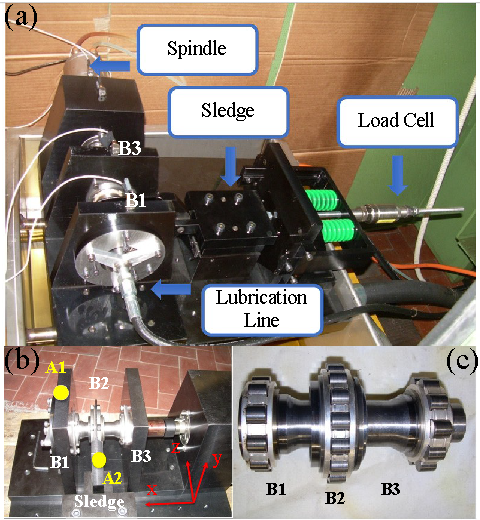
\includegraphics[width=0.65\linewidth]{figs/DRIG_test_rig.pdf}}
\caption{The bearing test rigs: a) a comprehensive overview of the test rig; b) the positions of the accelerometers and the reference system; c) the shaft fitted with three roller bearings. }
\label{figDRIG}
\end{figure}

\begin{table}[h]
    \centering
    \caption{Data Composition of different fault and dimension}
    \begin{tabular*}{\linewidth}{@{\extracolsep{\fill}}cc@{}} \hline
        
         \textbf{Fault} & \textbf{Dimension (\(\mu m\))}\\ \hline
        
         No defect& - \\
        
         Indentation size on the inner ring& 450 \\
        
         Indentation size on the inner ring& 250 \\
        
         Indentation size on the inner ring& 150 \\
        
         Indentation size on a roller& 450 \\
        
         Indentation size on a roller& 250 \\
        
         Indentation size on a roller& 150 \\ \hline
        
    \end{tabular*}
\label{label}
\end{table}
\begin{table}[h]
    \centering
    \caption{Dataset under different rotating frequency}
    \begin{tabular*}{\linewidth}{@{\extracolsep{\fill}}ccc@{}} \hline
        
        \textbf{Frequency (Hz)} & \textbf{Data Shape} & \textbf{Label Shape} \\ \hline
        
        100 & (3375, 4096, 6) & (3375,1) \\
        
        200 & (3125, 4096, 6) & (3125,1) \\
        
        300 & (3500, 4096, 6) & (3500,1) \\
        
        400 & (2625, 4096, 6) & (2625,1) \\
        
        500 & (1750, 4096, 6) & (1750,1) \\ \hline
        
    \end{tabular*}
\label{WC}
\end{table}


\subsection{Compared methods}
In order to assess the performance of our model in terms of effectiveness, model explainability and diagnostic performance, we conduct a comparative analysis with various IFD methods using different parameters, as detailed in Table \ref{table.signaldomain}. Among these methods is the ResNet fashion method, a widely recognized convolutional neural network utilized in various domains, including IFD \cite{Wang2020}. For our comparison, we selected the ResNet-18 version as M1, serving as the neural fashion backbone. Additionally, we assessed a SincNet-style filter baseline \cite{ravanelli_interpretable_2019} as M2 and the WKN model \cite{Li2022} as M3, both of which incorporate sinc filters and maintain Morlet wavelet convolution expertise analogous to ResNet. Moreover, we included the MWA-CNN \cite{Wang2023}, which integrates the Discrete Wavelet Attention Layer, as M4 for evaluation purposes.


\subsection{Case 1}
% \subsection{Results and discussion}
\subsubsection{Ablation study}

Firstly, an ablation study is conducted to evaluate the effectiveness of the modules in EKD and the different effect of hyperparameter, as shown in Fig. \ref{fig:abalation}. The $x$-axis represents the learning rate $\lambda$, and the $y$-axis represents the L1-norm weight $\gamma$. It can be observed from Fig. \ref{fig:abalation} (a) that employing all components at $\lambda \in [1e-5,1e-1]$ and $\gamma \in [1e-5,1e-1]$ yields a good validation accuracy. Conversely, in Fig. \ref{fig:abalation} (b), without filter knowledge, the model requires more tuning to find suitable parameters. The training of the proposed XOA Block becomes more challenging in the absence of residual connections, as depicted in Fig. \ref{fig:abalation} (c). Without the knowledge of solving the envelope via the HT transform, subsequent features are harder to explore, as shown in Fig. \ref{fig:abalation} (d). Fig. \ref{fig:abalation} (e) indicates that if only Mean is used for information aggregation, similar to traditional deep learning networks, the model struggles to converge to good performance. Lastly, Fig. \ref{fig:abalation} (f) demonstrates the significant role played by Kurtosis.

\begin{figure}[htbp]
\centerline{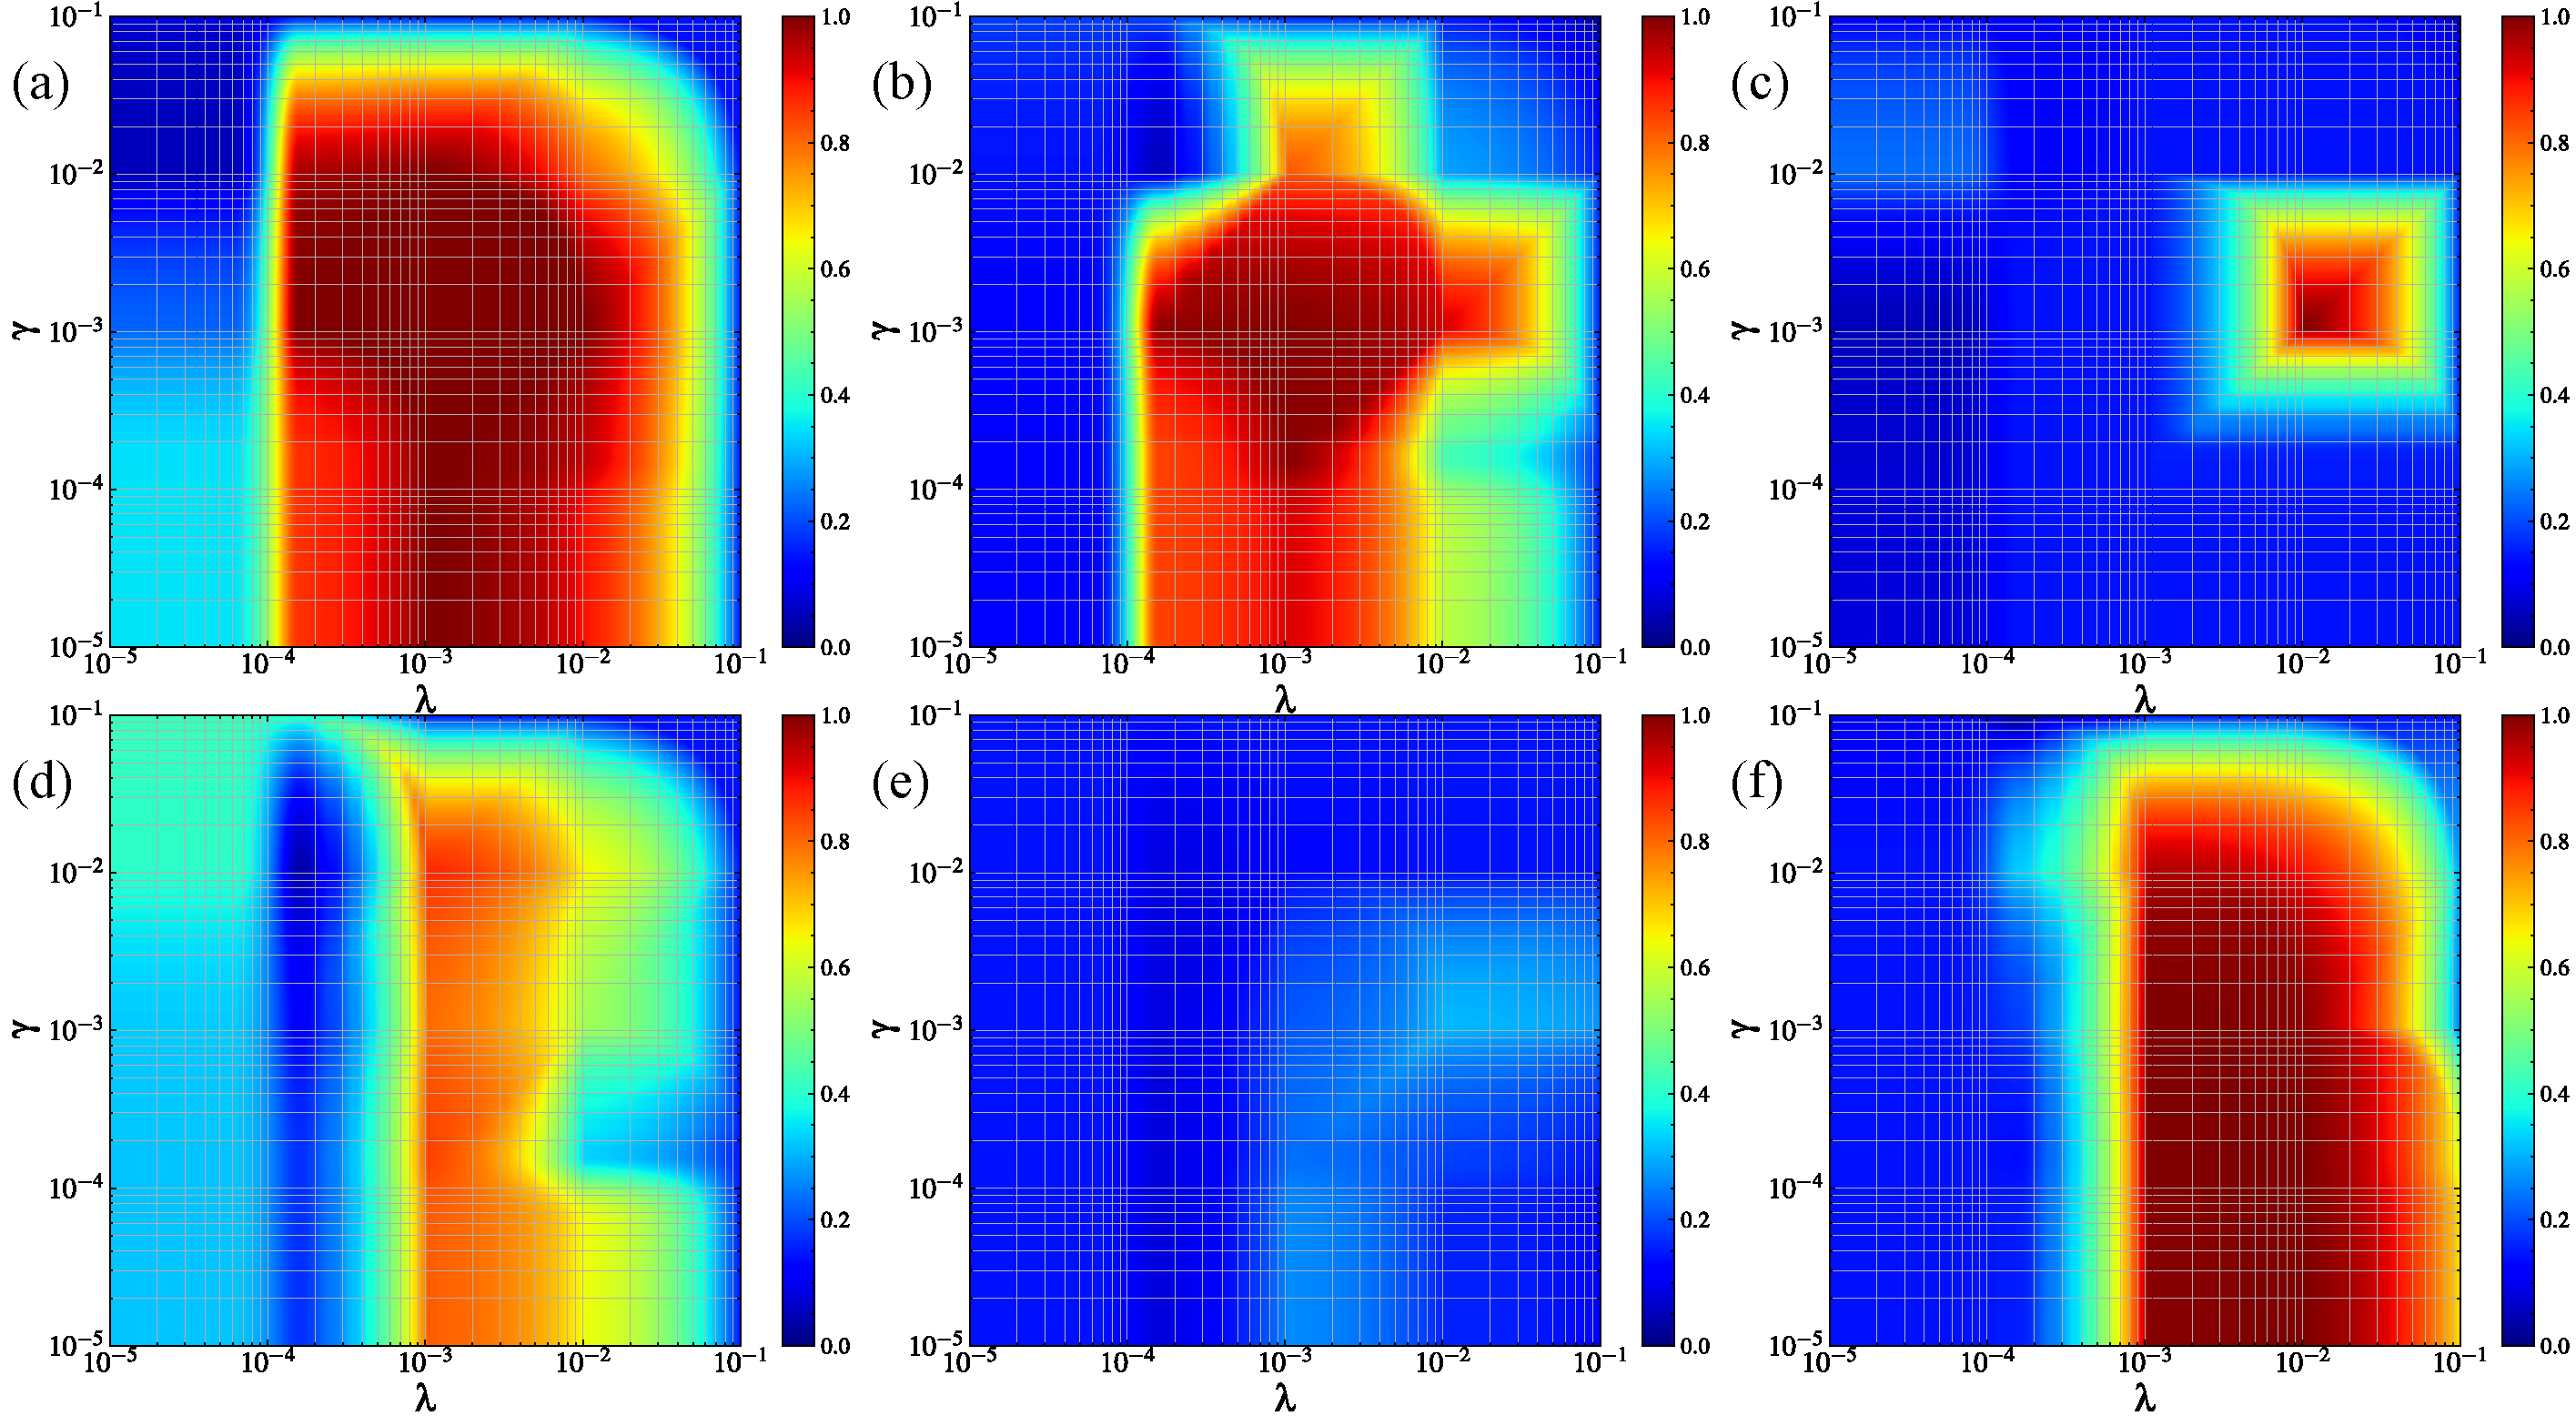
\includegraphics[width=1.0\linewidth]{figs/abalation.pdf}}
\caption{The ablation study.(a) all component, (b) w/o  wavelet filter, (C) w/o residule connection, (D) w/o  HT (e) only Mean , (f)  only Kurtosis.}
\label{fig:abalation}
\end{figure}



\subsubsection{Generalization results}


The XOAN method, with 34.37k parameters, demonstrates satisfactory performance with an accuracy of 100\% on D1T1 and 98.75\% ± 0.02\% on D1T2 which highlight the basic and generalization performance. This method is not only highly accurate but also explainable. The explainability feature suggests that XOAN can provide insights into how decisions are made, making it valuable for practical applications where understanding the decision-making process is crucial. Comparing XOAN to other methods, M1 has significantly more parameters (384.64k) but lacks explainability. Despite its complexity, M1 achieves a perfect score on D1T1 but performs poorly on D1T2, with an accuracy of only 52.38\% ± 4.17. This discrepancy highlights the importance of explainability and possibly a more efficient model architecture in achieving consistent performance across different datasets. Methods M2 and M3, both with 384.55k parameters and explainability features, achieve 100\% accuracy on D1T1 but show substantial variance and lower performance on D1T2 (50.34\% ± 23.34 and 61.86\% ± 19.38, respectively). Method M4, with 87.00k parameters and explainability, shows good performance on both datasets with accuracies of 97.61\% ± 4.21 on D1T1 and 96.05\% ± 2.77 on D1T2. Although M4 is explainable and performs well, it does not match the high consistency and accuracy of XOAN, particularly on D1T2.

\begin{table}
    \centering
\caption{Diagnosis accuracy of D1T1,D1T2.}
\label{table.signaldomain}
    \begin{tabular}{cclll} \hline  
         Methods&    Parameters& Explainability& D1T1 (\%)&D1T2 (\%)\\ \hline  
         XOAN& \textbf{34.37k}& $\checkmark$& 100$\pm$0&\textbf{98.75$\pm$0.02}\\ 
         M1& 384.64k& /& 100$\pm$0&52.38$\pm$4.17\\ 
         M2& 384.55k& $\checkmark$& 100$\pm$0&50.34$\pm$23.34\\ \hline
 M3& 384.55k& $\checkmark$& 100$\pm$0&61.86$\pm$19.38\\
 M4& 87.00k& $\checkmark$& 97.61$\pm$4.21&96.05$\pm$2.77\\  \hline
    \end{tabular}
\end{table}




\subsubsection{Explainable insights}

Fig. \ref{fig.attention_vis_1} to Fig. \ref{fig.attention_vis_15} illustrate ASs at various levels under three distinct working conditions in the D1T2 task. These figures demonstrate that XOAN provides explainable insights by adaptively highlighting key channels and discriminative operator groups from EKD across different samples and categories. The distribution and accumulation of ASs reveal the significant features that the model emphasizes, offering researchers valuable explainable information.



\textbf{Overall, the DSOA demonstrates adaptive attention towards explainable operators.}
In Fig. \ref{fig.attention_vis_10} (a), the ASs between different samples and various operator channels are displayed. The color intensity represents the AS magnitude, with darker colors indicating higher scores and lighter colors indicating lower scores. This figure shows that different samples focus on different operator channels, demonstrating the ability to adaptively highlight significant operators for different samples. 

\textbf{Discriminative Operator Group Selection for Enhanced Classification.}
Fig. \ref{fig.attention_vis_10} (b) shows the cumulative ASs for different operator groups across various channels. These groups use one type of operator multiple times. Each row represents a sample, and each column represents an operator group. The consistent selection of certain operator groups across multiple samples indicates their significant contribution to the classification process. 

\textbf{Category-Specific Attention Patterns in Feature Channels.}
Fig. \ref{fig.attention_vis_10} (c) depicts the cumulative ASs for samples of the same bearing health condition across different operator channels. Each row corresponds to a category, and each column represents an operator channel. This figure illustrates that samples within the same category tend to have high cumulative scores in specific feature channels, indicating high discriminative power of these operators for that category.

\textbf{Specific categories of signals exhibit specific preferences for interpretable operators.}
Fig. \ref{fig.attention_vis_10} (d) shows the accumulated number of non-zero attention between different categories and operators. Each row represents a category, and each column represents an operator group, i.e., specific operators in Table \ref{tab:feature sets}. This figure demonstrates that different categories tend to accumulate high scores in specific operator groups, highlighting the discriminative features for each category. 


\begin{figure}[htbp] 
\centerline{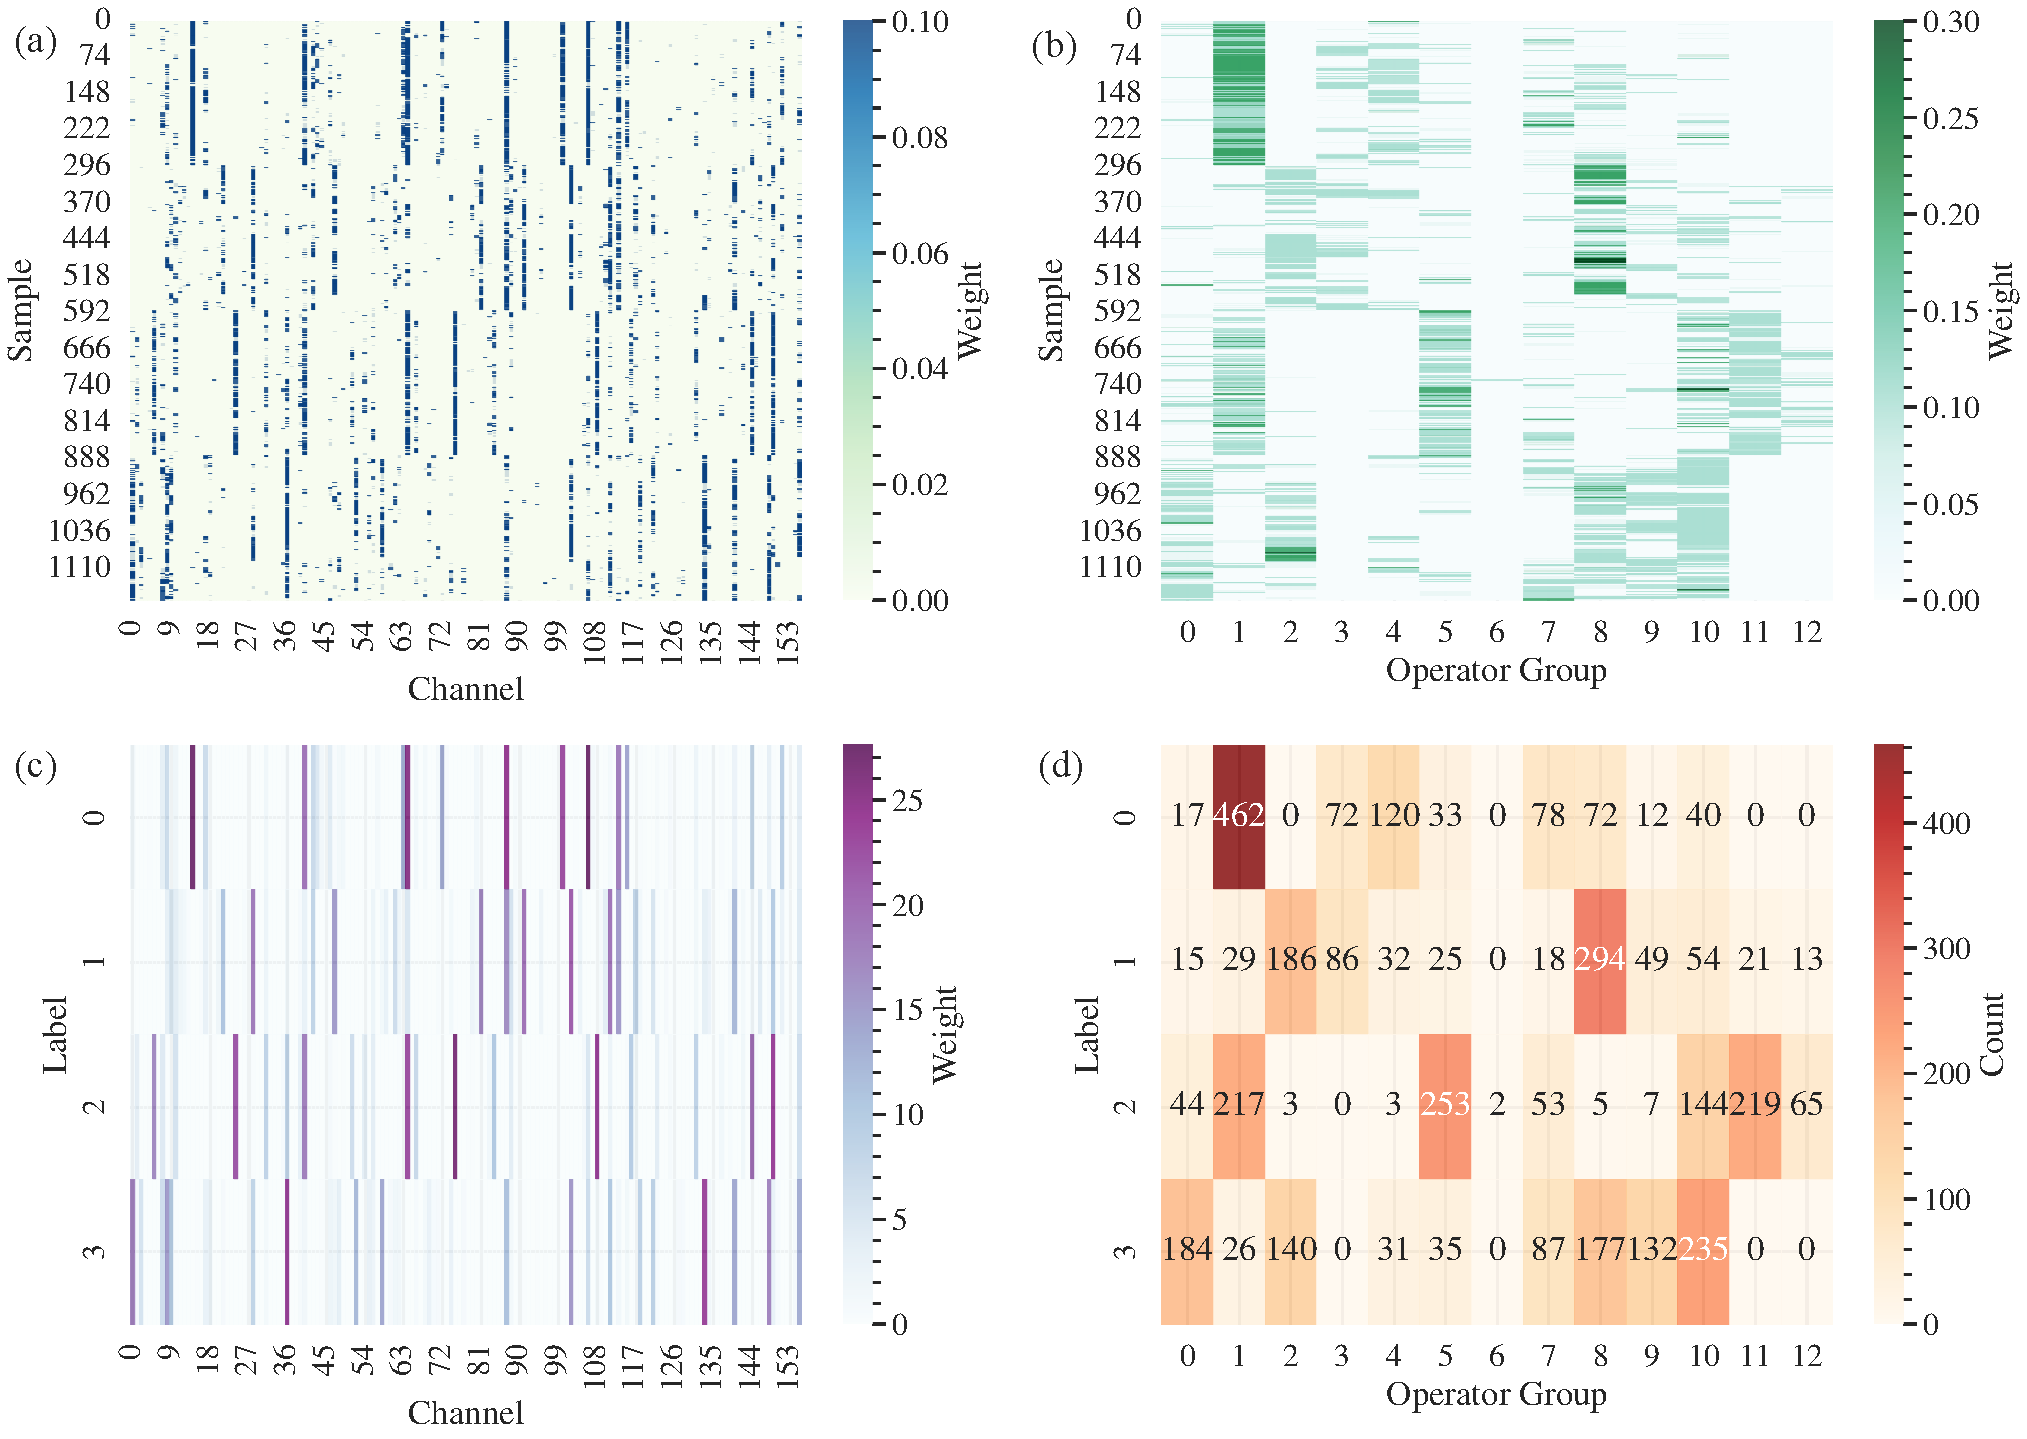
\includegraphics[width=1.0\linewidth]{figs/case1/AttentionFE_attnention1.pdf}}
\caption{ASs of operators under 1Hz, (a) scores across samples and channels, (b) accumulated scores across samples and operators, (c) accumulated scores per category across samples and channels, (d) accumulated non-zero attention number across categories and operators.}
\label{fig.attention_vis_1}
\end{figure}

\begin{figure}[htbp] 
\centerline{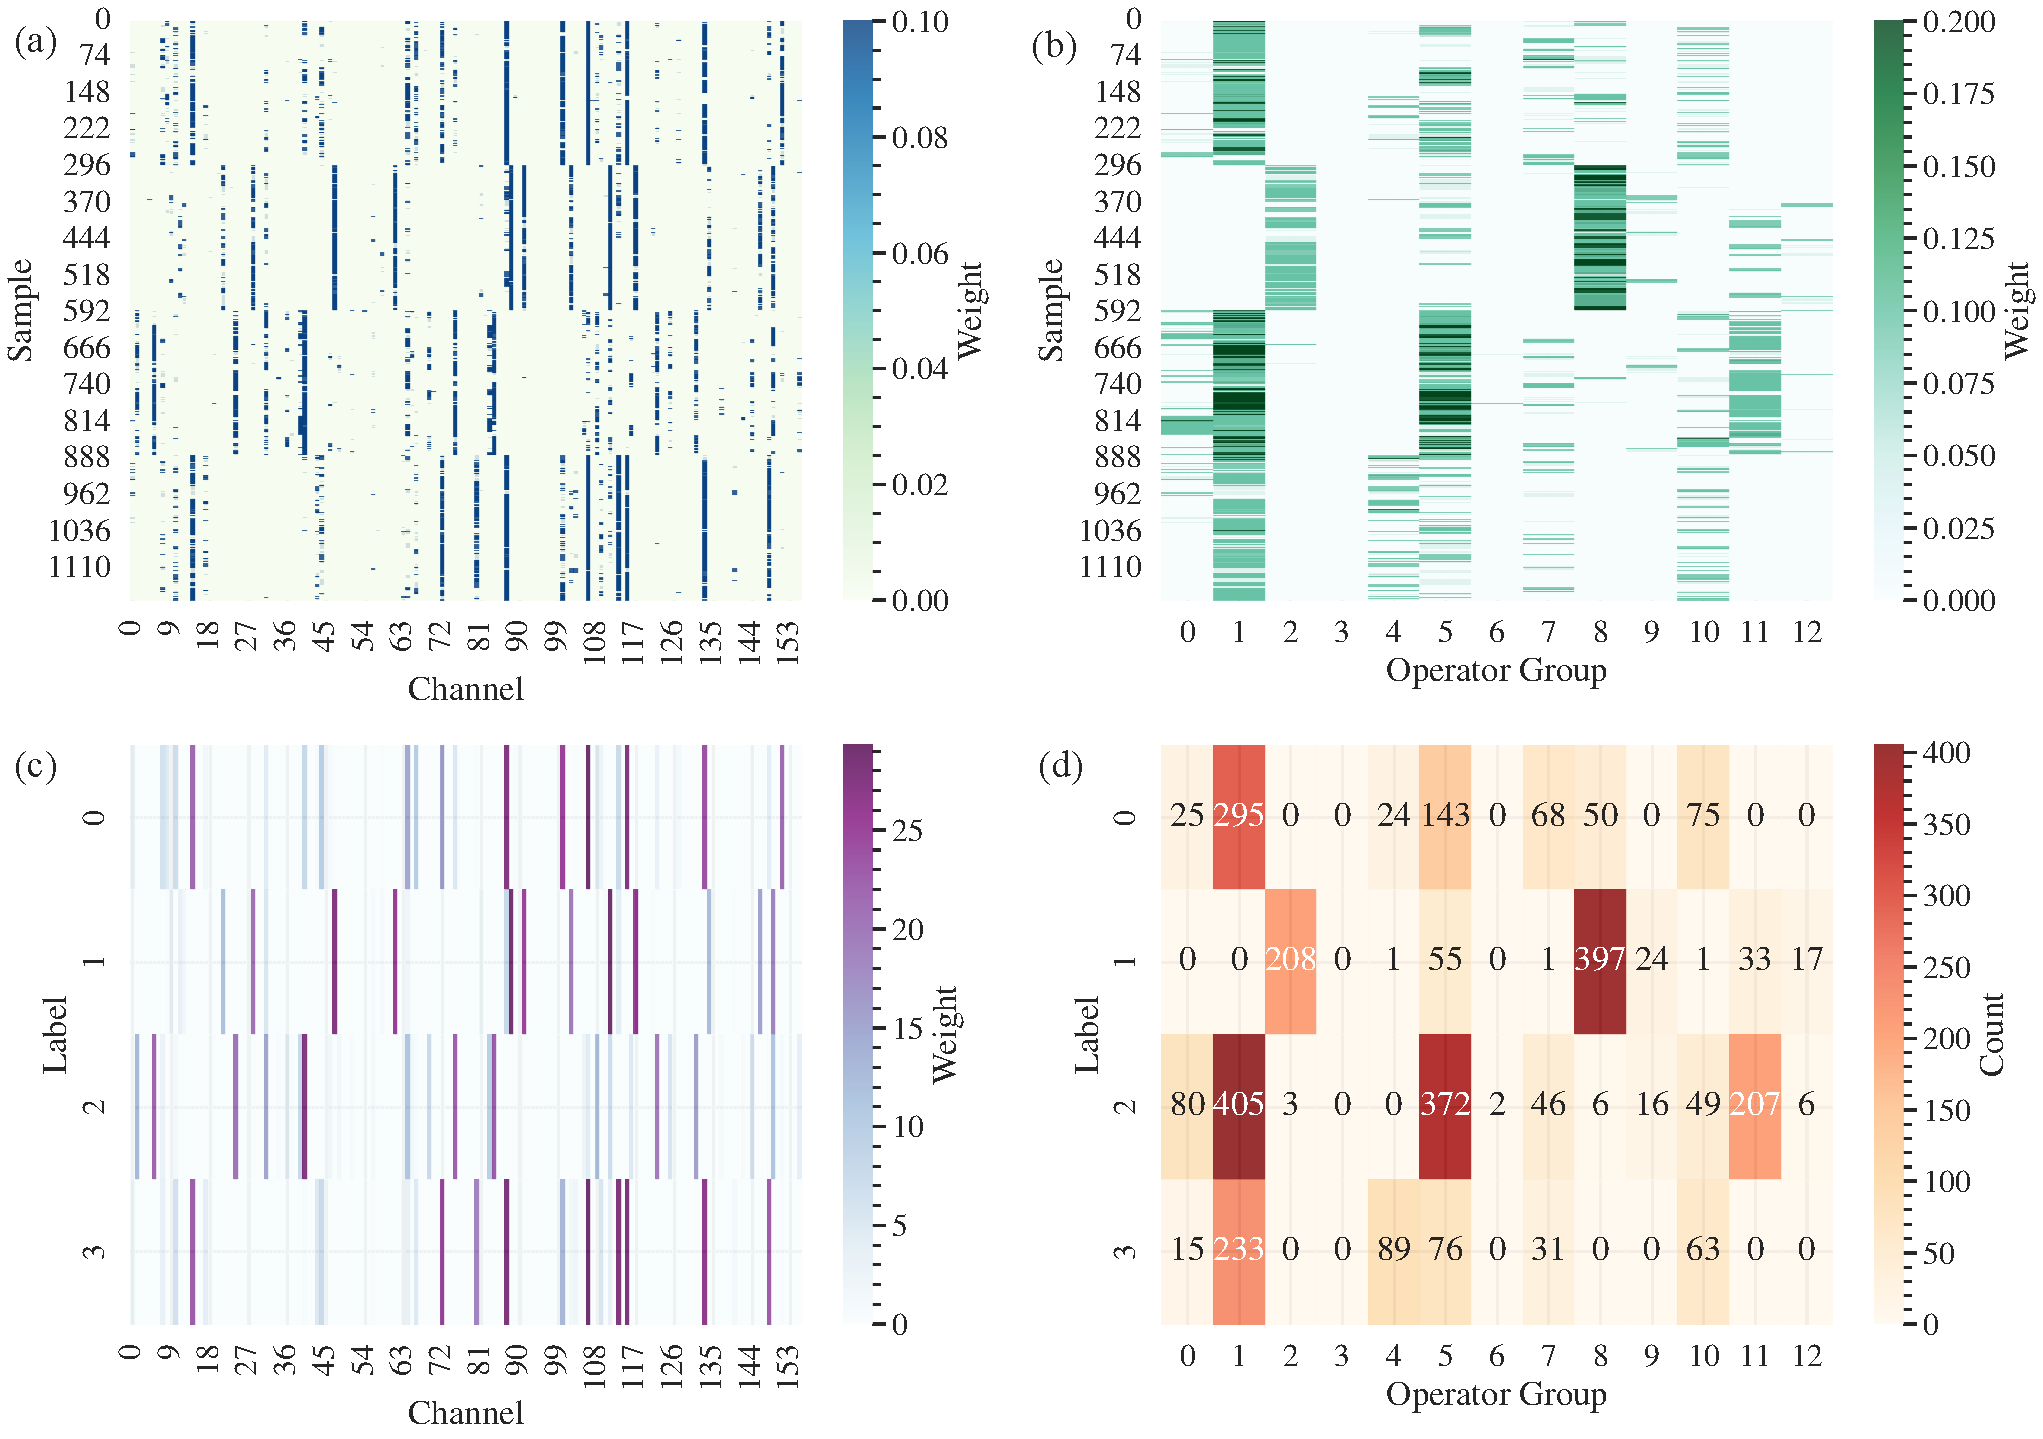
\includegraphics[width=1.0\linewidth]{figs/case1/AttentionFE_attnention10.pdf}}
\caption{ASs of operators under 10Hz, (a) scores across samples and channels, (b) accumulated scores across samples and operators, (c) accumulated scores per category across samples and channels, (d) accumulated non-zero attention number across categories and operators.}
\label{fig.attention_vis_10}
\end{figure}

\begin{figure}[htbp] 
\centerline{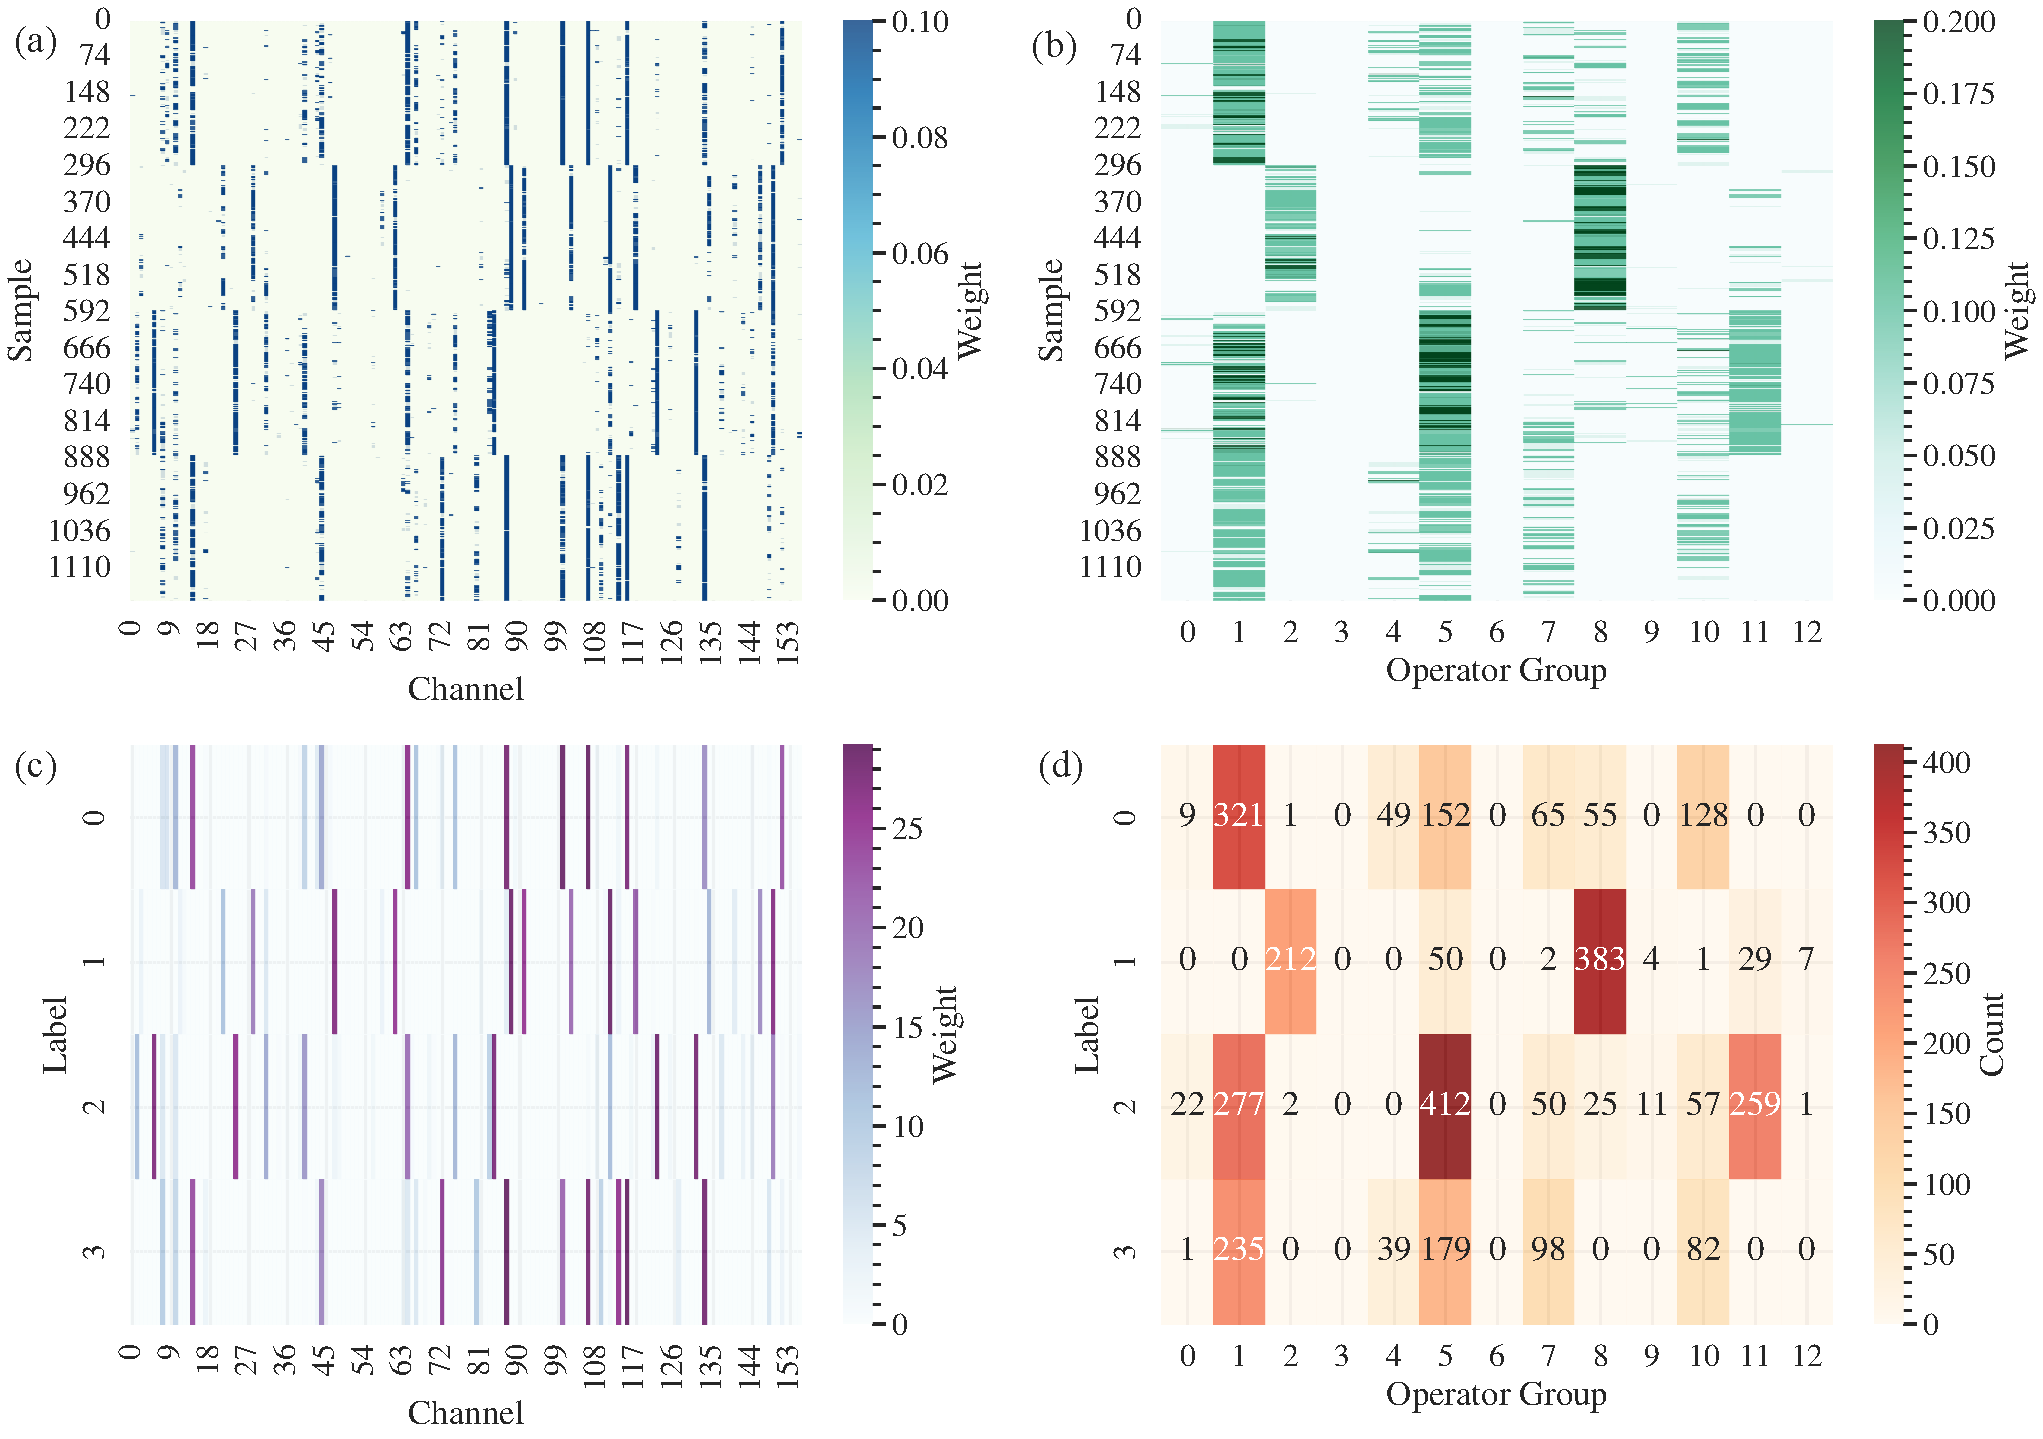
\includegraphics[width=1.0\linewidth]{figs/case1/AttentionFE_attnention15.pdf}}
\caption{ASs of operators under 15Hz, (a) scores across samples and channels, (b) accumulated scores across samples and operators, (c) accumulated scores per category across samples and channels, (d) accumulated non-zero attention number across categories and operators.}
\label{fig.attention_vis_15}
\end{figure}

\textbf{Varying feature preferences for different signal categories under different operating conditions.}
Training the model at 1Hz in Fig. \ref{fig.attention_vis_1} and 15Hz in Fig. \ref{fig.attention_vis_15} revealed that the model exhibited varying feature preferences for different signal categories under different operating conditions, which can aid researchers in post hoc optimization analysis. Specifically, at 1Hz, the model focused more on Std feature for normal samples, while for samples of IF, it emphasized RMS and variance. For samples of BF, the model paid closer attention to std, peak value, and clearance factor. For category 3 of OF, mean variance, RMS, and skewness were the prominent features. In contrast, the model tested at 15Hz in Fig. \ref{fig.attention_vis_15} showed different feature preferences for different signal categories. For normal signals, the focus was on standard deviation and peak value. In the case of  IF, Var and RMS were key features. When dealing with BF, Std, peak value, and clearance factor were highlighted. Lastly, for OF, Std, peak value, and Kurtosis value were significant. 

\textbf{Generalized features to unseen working conditions.}
When examining the model with samples at 10Hz, which it had not seen before training, it displayed similar feature preferences to those at 15Hz. This suggests that the model possesses the capability to adaptively focus on and select features based on different operating conditions and signal categories.


\subsubsection{Feature visualization} XOAN can adaptively extract features because DSOA has the capability to dynamically learn to select key operators. We use t-SNE visualization to show the evolution of features across the network as shown in Fig. \ref{fig.feature_tsne}. In Fig. \ref{fig.feature_tsne} (a), the features are exposed to rotational operational conditions, indicating domain separation. This is contradictory to our original intention of extracting domain-invariant features. Consequently, it is challenging to achieve optimal performance in one operating condition while performing well in another. Within each domain, data points associated with different labels are not clearly distinguished, leading to label confusion within the same domain. Fig. \ref{fig.feature_tsne} (b) illustrates the signal prior to DSOA in the initial $XOA_{SP}$ block. After undergoing processing by the signal operator, it can be observed that the distinguishability between inter-domains is limited. Fig. \ref{fig.feature_tsne} (c) demonstrates sparse attention, where a small number of features are highlighted to focus on specific signal operator nodes. Ultimately, by performing a dot product to obtain the signal solved by the attention operator, and after t-SNE dimensionality reduction, it is evident that although clustering primarily relies on domains for differentiation, there is some distinguishability among different feature categories within inter-domains.

Furthermore, after passing through multiple layers of $XOA_{SP}$ blocks, it is noticeable in Fig. \ref{fig.feature_tsne} (e) that the distinguishability between inter-domains gradually increases; however, interference from domains has not been fully addressed. Encouragingly, in Fig. \ref{fig.feature_tsne} (f), DSOA effectively distinguishes different features for various operating conditions, aiding in extracting domain-invariant features, as demonstrated in Fig. \ref{fig.feature_tsne} (e). Finally, Fig. \ref{fig.feature_tsne} (h) depicts the output features, indicating that even without utilizing specific domain generalization strategies, domain-invariant features can still be extracted.

\begin{figure}[htbp] 
\centerline{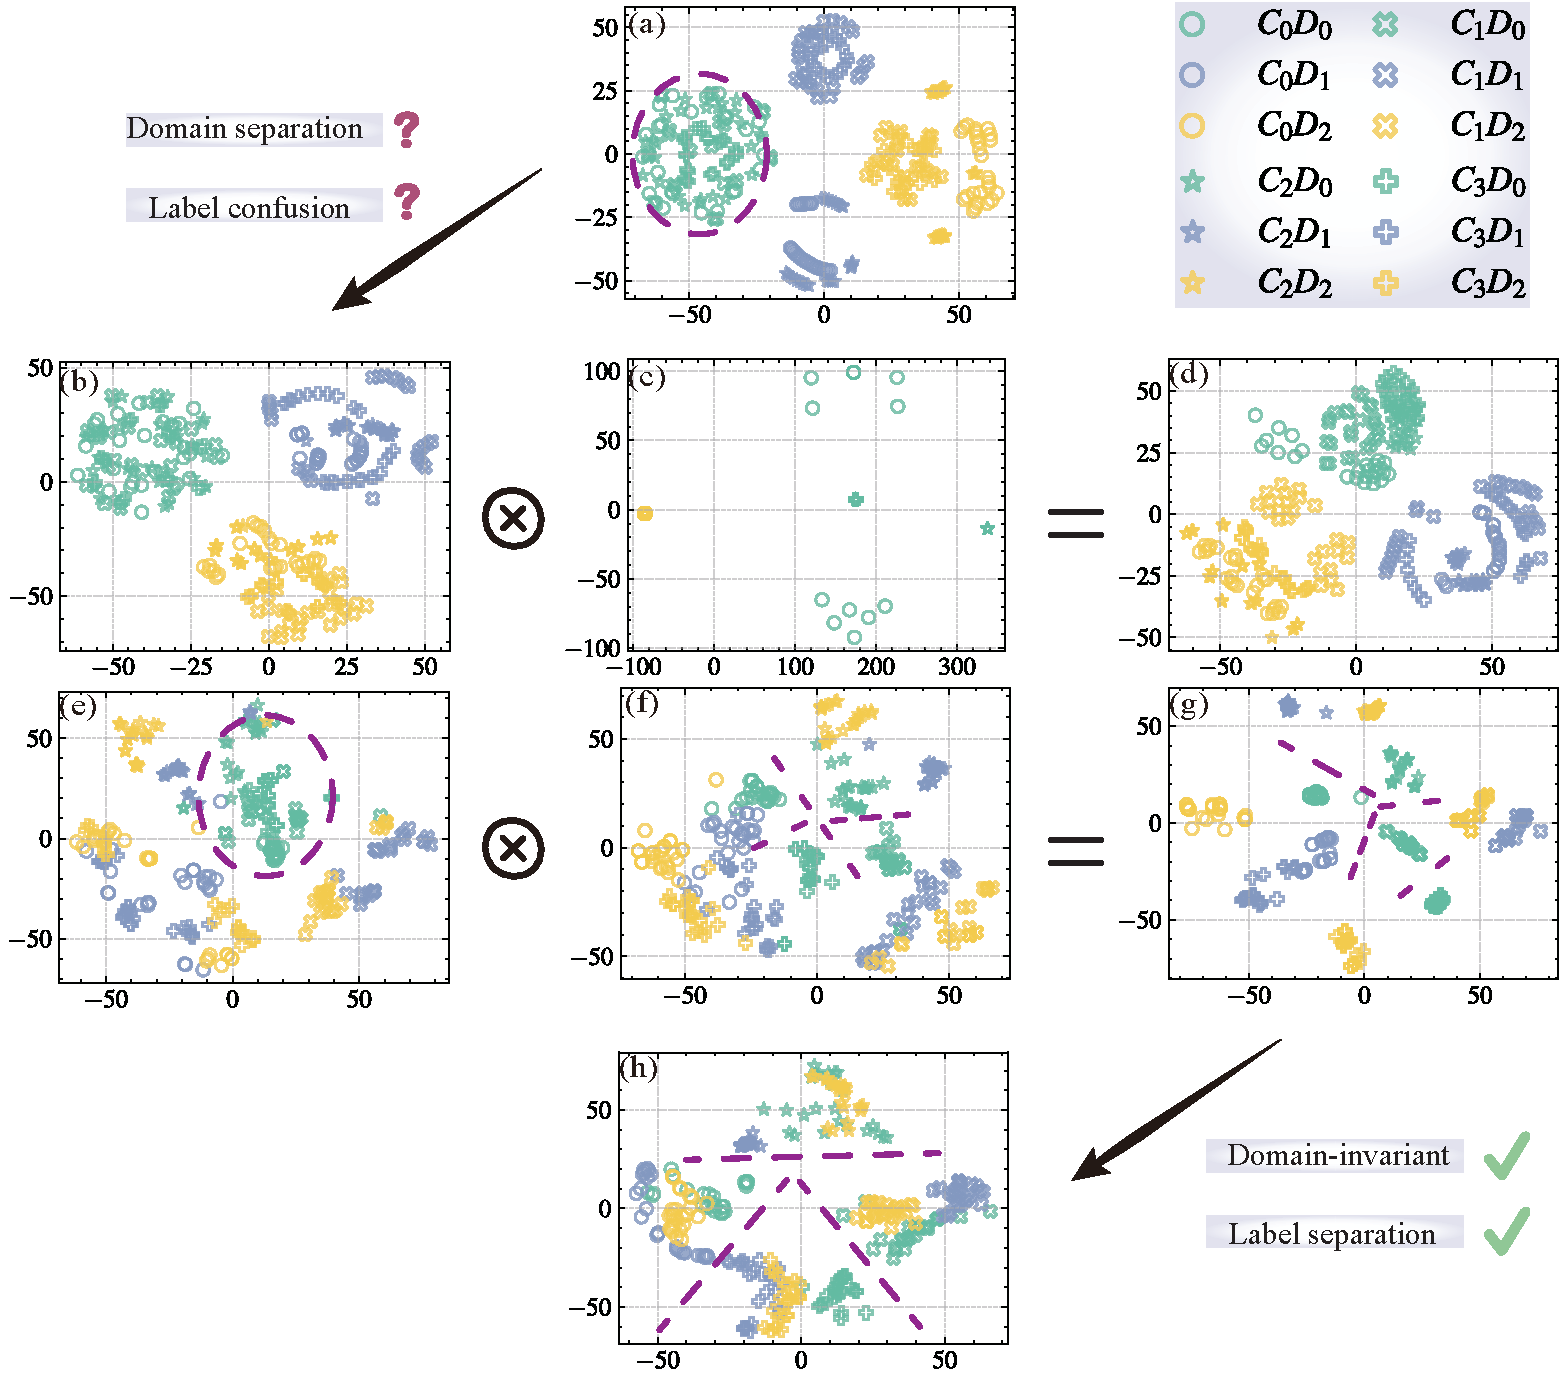
\includegraphics[width=1.0\linewidth]{figs/case1/feature_case1_short.pdf}}
\caption{t-SNE visualization shows the evolution of features across the network. The sequence includes the features of: (a) original signal, (b) signal prior to DSOA in the initial $XOA_{SP}$ block, (c) DSOA in the initial $XOA_{SP}$ block, (d) signal after DSOA in the initial $XOA_{SP}$ block, (e) signal before DSOA in the $XOA_{FE}$ block, (f) DSOA in the $XOA_{FE}$ block, (g) signal after DSOA in the $XOA_{FE}$ block, and (h) output signal.}
\label{fig.feature_tsne}
\end{figure}


\subsection{Case 2}

% \subsubsection{basic} % TODO

% \begin{table}
%     \centering
% \caption{Diagnosis accuracy of D2T1,D2T2,D2T3.}
% \label{table.signaldomain}
%     \begin{tabular}{cclll} \hline  
%          Methods&    Parameters& Interpretability& D2T1 (\%)&D2T2 (\%)\\ \hline  
%          XOAN& \textbf{34.37k}& $\checkmark$& 100$\pm$0&\textbf{98.75$\pm$0.02}\\ 
%          M1& 384.64k& /& 100$\pm$0&52.38$\pm$4.17\\ 
%          M2& 384.55k& $\checkmark$& 100$\pm$0&50.34$\pm$23.34\\ \hline
%  M3& 384.55k& $\checkmark$& 100$\pm$0&61.86$\pm$19.38\\
%  M4& 87.00k& $\checkmark$& 100$\pm$0&96.05$\pm$2.77\\  \hline
%     \end{tabular}
% \end{table}

\subsubsection{Diagnosis performance under noise attack} \label{c.snr_curve}

Fig. \ref{fig_noise} illustrates the performance comparison of different methods in combating varying levels of noise. It can be observed that the proposed approach exhibits comparable performance to the M1, M3 and M4 methods under low noise conditions, approaching higher levels of accuracy. As the noise levels increase, the accuracy of all models is affected, leading to a decline. The proposed method, by integrating the interpretability of expert knowledge with the adaptability of neural networks, further enhances the robustness of the model.

\begin{figure}[htbp]
\centerline{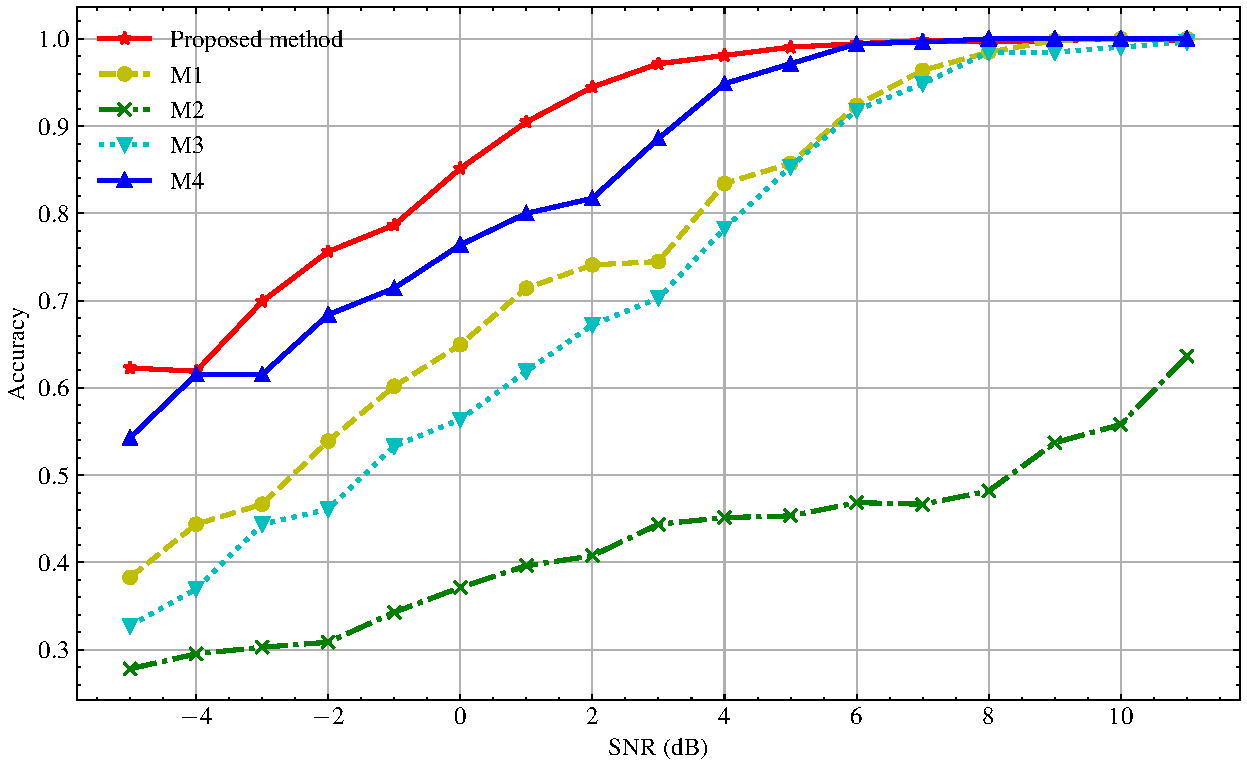
\includegraphics[width=0.95\linewidth]{figs/case2/accuracy_vs_snr_case2.pdf}}
\caption{The robustness of different methods under different noise.}
\label{fig_noise}
\end{figure}

\subsubsection{AS under noise attack} When observing the characteristics of attention in dynamic recognition models without noise in Fig. \ref{fig.attention_vis_case2}, it is evident that healthy samples exhibit low attention to features. Kurtosis emerges as a significant feature, particularly for identifying slight faults in the peak value and kurtosis of the IF fault. In cases of moderate faults in the IF, Variance, Entropy, and kurtosis play crucial roles. Moreover, for severe IF faults, Crest Factor and Clearance Factor are notably important features. In the context of faults in the OF fault, slight faults are notably valuable for Std and peak value. Moderate faults are characterized by standard deviation, entropy, Crest Factor, and Clearance Factor. Severe faults are distinguished by mean, peak value, Crest Factor, and Clearance Factor as key features.
Furthermore, in Fig. \ref{fig.attention_vis_case2_noise}, the model still maintains a relatively high accuracy. At this point, the model predominantly focuses on Kurtosis and clearance Factor as key features, indicating their strong noise robustness, which aligns with expert knowledge. Therefore, the proposed method effectively integrates expert knowledge and neural networks, enhancing the performance of model.

\begin{figure}[htbp] 
\centerline{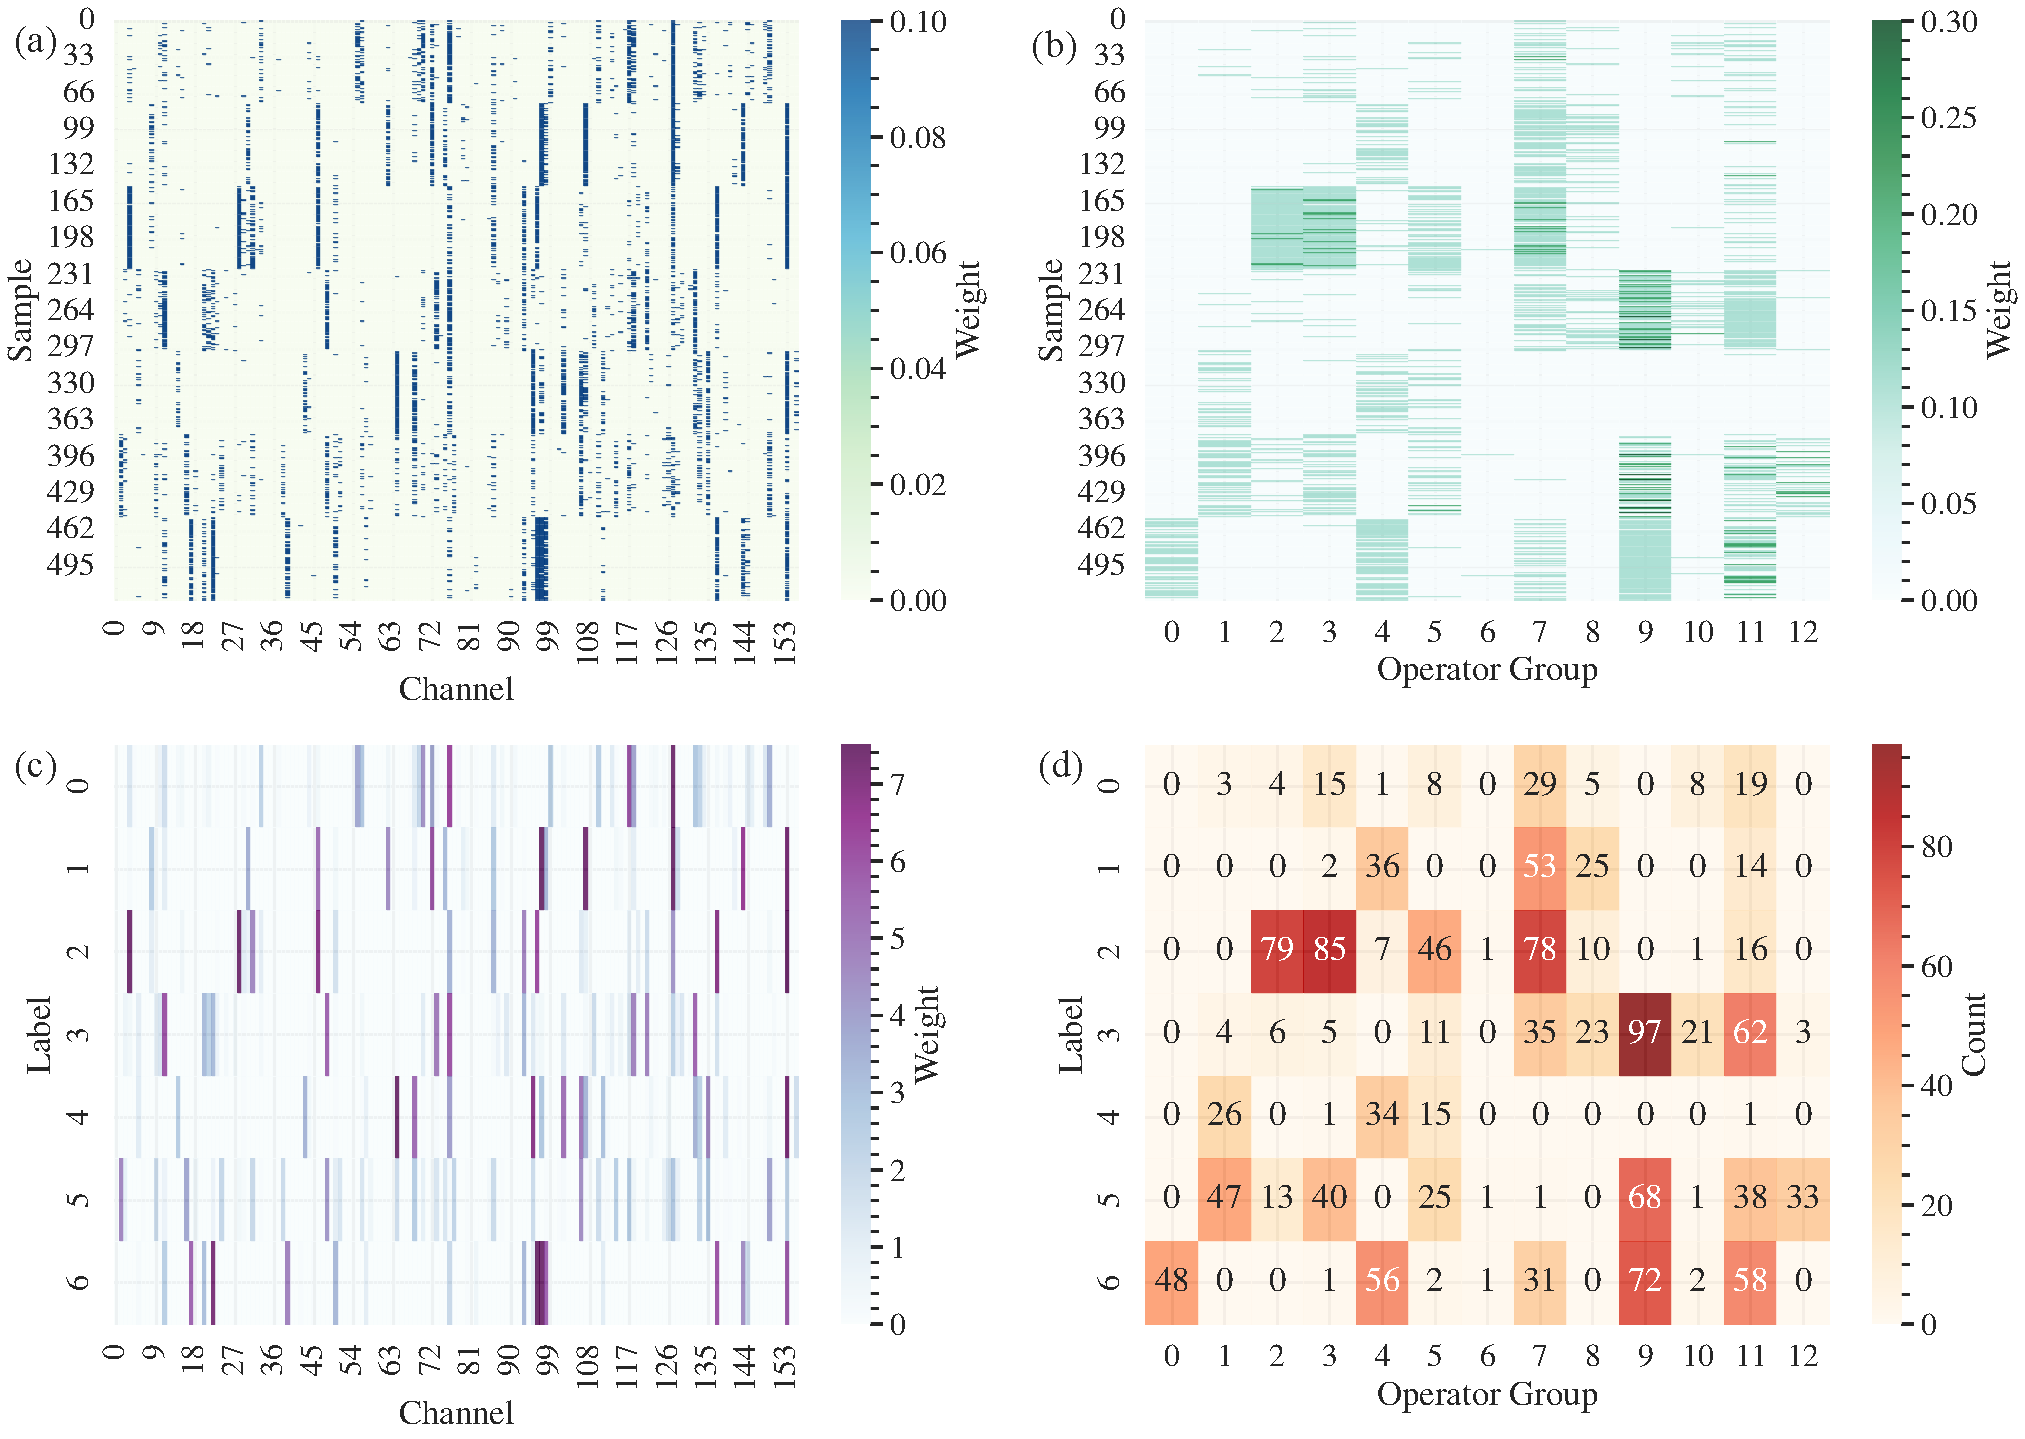
\includegraphics[width=1.0\linewidth]{figs/case2/AttentionFE_attnention.pdf}}
\caption{AS of features without noise, (a) Scores across samples and channels, (b) Accumulated scores across samples and operator, (c) Accumulated scores per category across samples and channels, (d) Accumulated scores across categories and operator.}
\label{fig.attention_vis_case2}
\end{figure}


\begin{figure}[htbp] 
\centerline{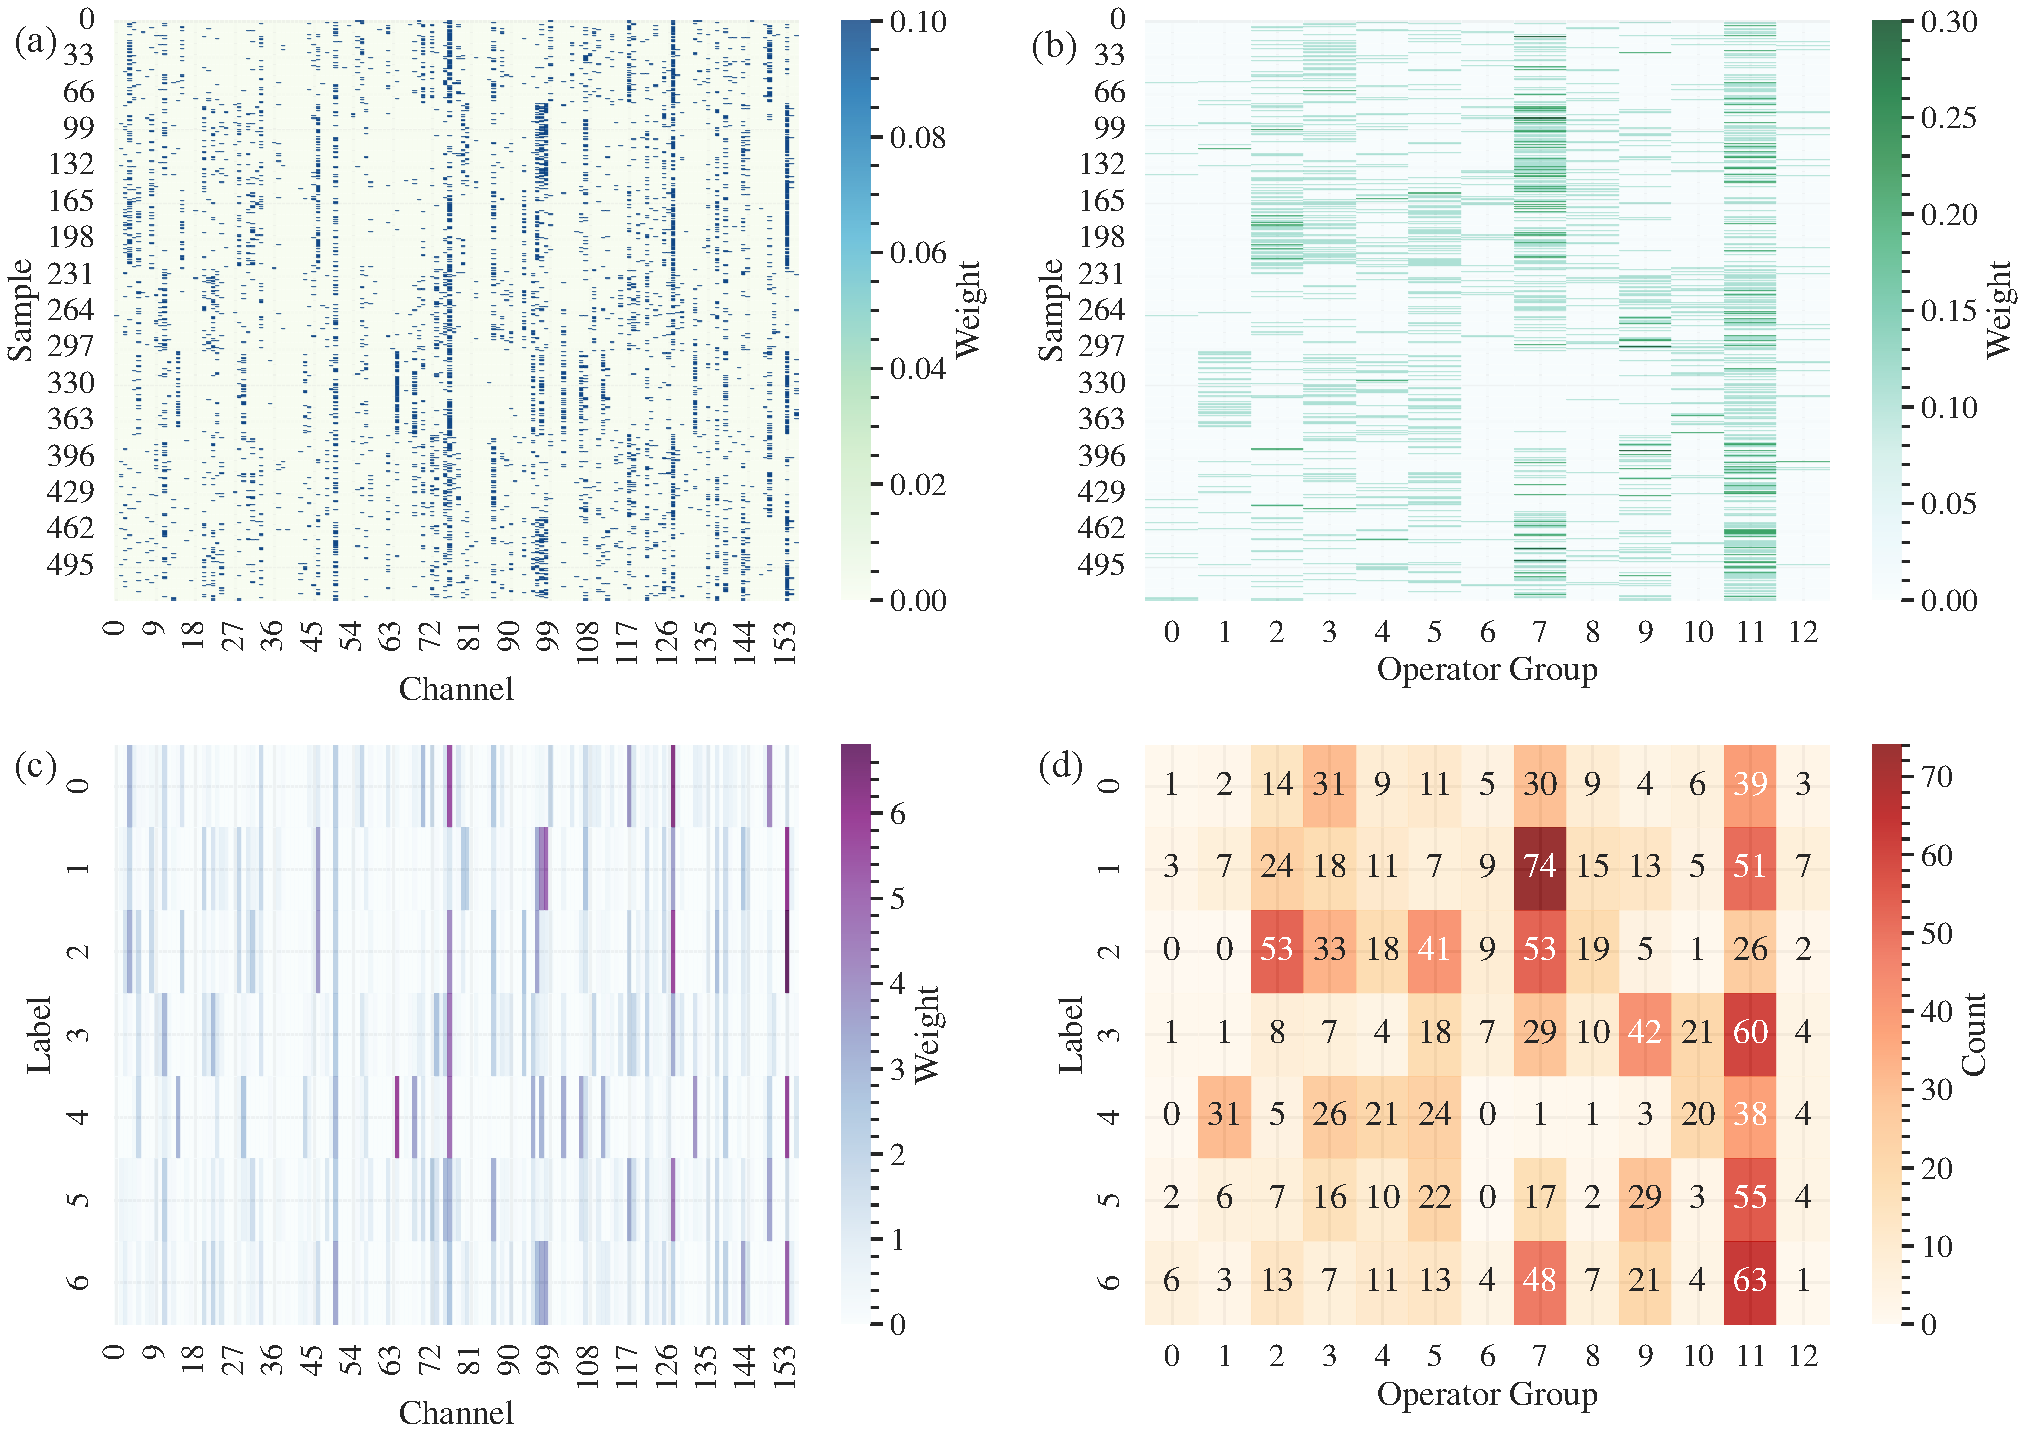
\includegraphics[width=1.0\linewidth]{figs/case2/AttentionFE_attnention_noise.pdf}}
\caption{AS of features with 0db noise, (a) Scores across samples and channels, (b) Accumulated scores across samples and operator, (c) Accumulated scores per category across samples and channels, (d) Accumulated scores across categories and operator.}
\label{fig.attention_vis_case2_noise}
\end{figure}


% \subsubsection{gen}

\section{Conclusion}

This study proposes the eXplainable Operator Attention Network (XOAN) to dynamically learn and utilize expert knowledge for bearing fault diagnosis, aiming to enhance the explainability and adaptability of intelligent diagnostic models. The XOAN integrates an Expert Knowledge Dictionary (EKD) and Dynamic Sparse Operator Attention (DSOA) to adaptively identify features. Through a case study, it is shown that XOAN not only achieves satisfactory diagnostic performance but also offers insights into selecting operators for more effective diagnostics using DSOA mechanisms. The effectiveness of the modules is verified through ablation studies, while attention scores reveal the utilization of expert knowledge, and feature visualization demonstrates the adaptive selection of operators and extraction of interpretable features based on different operating conditions, offering significant benefits for industrial applications. 

Future research will focus on expanding the EKD with criteria for selecting and conducting more extensive tests with additional data and diagnostic tasks to further enhance the applicability of DSOA and XOAN.

% Through two case studies,



\bibliographystyle{IEEEtran}
\bibliography{ref.bib}



% \section*{Acknowledgments}
% This should be a simple paragraph before the References to thank those individuals and institutions who have supported your work on this article.







%{\appendices
%\section*{Proof of the First Zonklar Equation}
%Appendix one text goes here.
% You can choose not to have a title for an appendix if you want by leaving the argument blank
%\section*{Proof of the Second Zonklar Equation}
%Appendix two text goes here.}



% \section{References Section}
% You can use a bibliography generated by BibTeX as a .bbl file.
%  BibTeX documentation can be easily obtained at:
%  http://mirror.ctan.org/biblio/bibtex/contrib/doc/
%  The IEEEtran BibTeX style support page is:
%  http://www.michaelshell.org/tex/ieeetran/bibtex/
 
%  % argument is your BibTeX string definitions and bibliography database(s)
% %\bibliography{IEEEabrv,../bib/paper}
% %
% \section{Simple References}
% You can manually copy in the resultant .bbl file and set second argument of ∖\backslash{\tt{begin}} to the number of references
%  (used to reserve space for the reference number labels box).

% \begin{thebibliography}{1}
% \bibliographystyle{IEEEtran}
% \bibliography{UPHM.bib}


% \end{thebibliography}

%#############################################################################################

% \begin{IEEEbiography}[{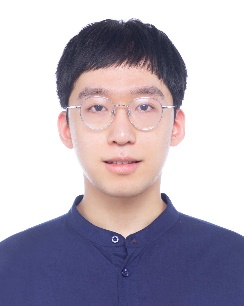
\includegraphics[width=1in,height=1.25in,clip,keepaspectratio]{figs/Author_Qi_Li.png}}]{Qi Li}received the B.Eng. and M.Eng. degrees in electrical engineering and control theory and control engineering from Soochow University, Suzhou, China, in 2019 and 2022, respectively.

% He is currently pursuing the Ph.D. degree in mechanical engineering with Tsinghua University, Beijing, China. His research interests lie in the intersection of trustworthy AI, reliable prognostic and health management (PHM) and foundation models.
% \end{IEEEbiography}

% \begin{IEEEbiography}[{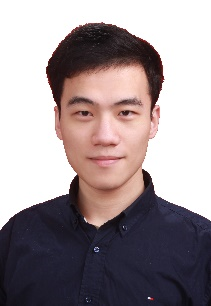
\includegraphics[width=1in,height=1.25in,clip,keepaspectratio]{figs/Author_Wenyang_Hu.png}}]{Wenyang Hu} was born in Changsha, China, in 1998. He received the B.S. degree in mechanical engineering and automation from Central South University (CSU), Changsha, China, in 2020. 

% He is now a Ph.D. candidate in the Department of Mechanical Engineering, Tsinghua University, China. His research interests include digital twins, fault diagnosis and prognostics of mechatronics equipment, and signal processing.
% \end{IEEEbiography}
% % \begin{IEEEbiography}[{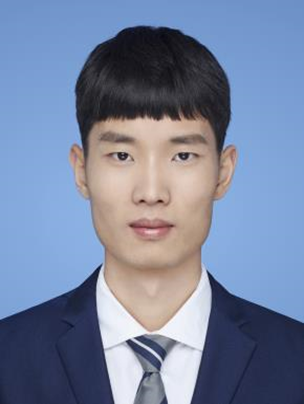
\includegraphics[width=1in,height=1.25in,clip,keepaspectratio]{figs/Author_Shilin_Sun.png}}]{Shilin Sun} was born in Linyi, China. He received the B.Eng. degree in transportation equipment and control engineering from Central South University, Changsha, China in 2019.

% % He is currently working toward the Ph.D. degree in mechanical engineering with Tsinghua University, Beijing, China. His research interests include condition monitoring and damage identification of machinery.
% % \end{IEEEbiography}

% \begin{IEEEbiography}[{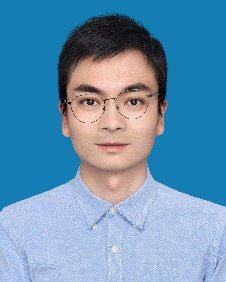
\includegraphics[width=1in,height=1.25in,clip,keepaspectratio]{figs/Author_Hua_Li.png}}]{Hua Li (M’19-)} was born in Zigong City, China, in 1988. He received the B.S. degrees in mechanical engineering from the North University of China, Taiyuan, China, in 2011. and the Ph. D. degree at faculty of mechanical and electrical engineering, Kunming University of Science and Technology in 2020. He has been a member of IEEE since 2019. Now he is a distinguished professor and master tutor of the State Key Laboratory of Public Big Data, Guizhou University, and also with the Department of Mechanical Engineering, Tsinghua University, Beijing 100084, China.

% So far, he has made some achievements in his field of interest. He has authored and coauthored more than 20 articles. His research interests include electromechanical system fault diagnosis, modern signal processing, structural health monitoring, image processing, machine learning, etc. He has a strong passion and a rigorous attitude for scientific research. His goal is to commit himself to better research.
% \end{IEEEbiography}

% \begin{IEEEbiography}[{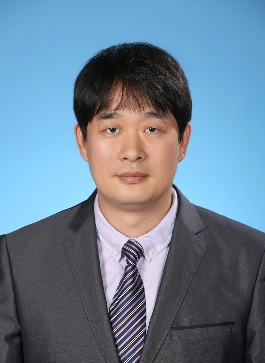
\includegraphics[width=1in,height=1.25in,clip,keepaspectratio]{figs/Author_Zhaoye_Qin.png}}]{Zhaoye Qin} received the B.S. and M.S. degrees in mechanical engineering from the School of Mechanical Engineering, Northeastern University, Shenyang, China, in 2003 and 2006, respectively, and the Ph.D. degree in mechanical engineering from the Department of Precision Instrument, Tsinghua University, Beijing, China, in 2010. 

% He is currently an Associate Professor with the Department of Mechanical Engineering, Tsinghua University, Beijing, China. His research interests include rotating machinery dynamics, machinery condition monitoring and fault diagnosis, shock and vibration control, energy harvesting, and nanocomposites.
% \end{IEEEbiography}
% \begin{IEEEbiography}[{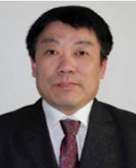
\includegraphics[width=1in,height=1.25in,clip,keepaspectratio]{figs/Author_Fulei_Chu.png}}]{Fulei Chu} received the B.Eng. degree in mechanical engineering from the Jiangxi University of Science and Technology, Ganzhou, China, in 1982, the M.Eng. degree in applied mechanics from Tianjin University, Tianjin, China, in 1985, and the Ph.D. degree in mechanical engineering from the University of Southampton, Southampton, U.K., in 1994.

% He is currently a Professor with the Department of Mechanical Engineering, Tsinghua University, Beijing, China. He has authored over 300 academic articles in the field of machinery dynamics, fault diagnosis, and vibration control.

% Prof. Chu is the Vice President of the Chinese Society for Vibration Engineering (CSVE), the Chairman of Fault Diagnostics Division in CSVE, and a member of the Technical Committee of Rotor Dynamics in the International Federation for Promotion of Mechanism and Machine Sciences (IFToMM). He was a recipient of the Second Prize of National Natural Science Award in 2003, the National Science Fund for Distinguished Young Scholars in 2004, the Second Prize of Natural Science Award of Ministry of Education in 2006, the First Prize of Natural Science Award of Ministry of Education in 2011, and the Prize of the International Society for Condition Monitoring in 2018.




% \end{IEEEbiography}

%###############################################


% \newpage

% \section{Biography Section}
% If you have an EPS/PDF photo (graphicx package needed), extra braces are
%  needed around the contents of the optional argument to biography to prevent
%  the LaTeX parser from getting confused when it sees the complicated
%  ∖\backslash{\tt{includegraphics}} command within an optional argument. (You can create
%  your own custom macro containing the ∖\backslash{\tt{includegraphics}} command to make things
%  simpler here.)
 
% \vspace{11pt}

% \bf{If you include a photo:}\vspace{-33pt}
% \begin{IEEEbiography}[{\includegraphics[width=1in,height=1.25in,clip,keepaspectratio]{fig1}}]{Michael Shell}
% Use $\backslash${\tt{begin\{IEEEbiography\}}} and then for the 1st argument use $\backslash${\tt{includegraphics}} to declare and link the author photo.
% Use the author name as the 3rd argument followed by the biography text.
% \end{IEEEbiography}

% \vspace{11pt}

% \bf{If you will not include a photo:}\vspace{-33pt}
% \begin{IEEEbiographynophoto}{John Doe}
% Use $\backslash${\tt{begin\{IEEEbiographynophoto\}}} and the author name as the argument followed by the biography text.
% \end{IEEEbiographynophoto}


\vfill

\end{document}
